\documentclass[12pt,letterpaper,table,svgnames,dvipsnames]{article}

% \begin{preamble}
\usepackage[margin=1in]{geometry}
\usepackage{times}

\usepackage{apacite}
% \usepackage{dblfloatfix}
\usepackage{caption}
\usepackage{subcaption}
\usepackage{graphicx}
\usepackage{tcolorbox}
% \usepackage{multicol}
\usepackage{makecell}
\usepackage{xcolor}
\usepackage{gb4e}
\noautomath
\usepackage{booktabs}
\usepackage{url}
% \end{preamble}

\definecolor{Purple}{RGB}{255,10,140}
\newcommand{\jd}[1]{\textcolor{Purple}{[jd: #1]}}
\newcommand{\mm}[1]{\textcolor{teal}{[mm: #1]}}
\newcommand{\tableref}[1]{Table~\ref{#1}}
\newcommand{\figref}[1]{Fig.~\ref{#1}}
\newcommand{\expref}[1]{Exp.~#1}
\newcommand{\whq}{\emph{wh}-question~}
\newcommand{\whqs}{\emph{wh}-questions~}
\newcommand{\whw}{\emph{wh}-word~}
\newcommand{\whws}{\emph{wh}-words~}

\newcommand{\ap}{\emph{a}~}
\newcommand{\everyp}{\emph{every}~}
\newcommand{\thep}{\emph{the}~}


\title{Who thinks questions are exhaustive? \\ A corpus experimental look at the semantics and pragmatics of \whqs}
\author{Morgan Moyer and Judith Degen}
\date{\today}

\begin{document}

\maketitle

\section{Introduction}

Consider that \whqs can be answered in multiple ways:
% \vspace{-.3cm}
\begin{exe}
    \ex {}
    \begin{xlist}
        \ex Where can I find coffee? \label{coffee1}
        % \vspace{-.1cm}
        \ex Who came to the party? \label{party}
    \end{xlist}
\end{exe}
% \vspace{-.3cm}
At first blush, the most natural way to answer (\ref{coffee1}) is to mention a nearby coffee shop, while the most natural way to answer (\ref{party}) is to provide an exhaustive list of party-goers. Thus, (\ref{coffee1}) is interpreted non-exhaustively while (\ref{party}) is interpreted exhaustively. We refer to these interpretations as `Mention-Some' (MS) and `Mention-All' (MA), respectively, following \citeA{hintikka1976,groenstok1982,groenstok1984}. \emph{Wh}-questions do not specify on the surface whether they are intended to be MS or MA. So what makes (\ref{coffee1}) MS, and what makes (\ref{party}) MA? The answer to that question is the focus of this paper.

On the one hand, it seems that MS is licensed in (\ref{coffee1}) by appeal to contextual goals (\cite{groenstok1982,groenstok1984}). If (\ref{coffee1}) is asked by a tourist whose goal is to drink a coffee, then a MS answer is felicitous; if asked by a coffee distributor whose goal is to explore the local market, then MA is felicitous. However, not all \whqs lend themselves to MS interpretations, while the MA interpretation appears to be available for most (if not all) \whqs. Indeed, (\ref{party}) is often presented as a paradigm \whq that does not allow MS.

Those works have focused typically on a small number of examples shared between researchers, on the implicit assumption that simple \whqs would not vary greatly. Recent work (\cite{moyersyrett2019,moyer2020}) has recruited larger-scaled experimental methods that systematically vary both linguistic and contextual factors across a broader range of sentence and context tokens, with the goal of creating a more stable empirical basis for a theory of \whq meaning. That work found evidence for a dual licensing of MS/MA by both the linguistic form of the questions and the contextual speaker goal. 

In the current study, we aim to contribute to the goal of broadening the empirical base through a large-scale study of naturalistic speech. We use a novel paraphrase rating task to estimate the acceptability of possible question paraphrases in root (Experiment 1a) and embedded (Experiment 1b) \whqs. These first studies presented participants with targets in the presence of the immediately preceeding discourse. In a second set of studies, we look at how the acceptability of possible paraphrases changes when the immediately preceeding discourse is removed (Experiments 2a and 2b). 

The picture that emerges is that there is considerable variation in question interpretation. That variation arises from (1) the contextual goals, (2) the uttered question, (3) the hearer's inferences about the two, and (4) any prior expectations that the hearer might have about either (1), (2), or (3). Together, with a more quantitaive analysis of the contribution of the preceeding discourse context we argue that accounting for \whq meaning in terms of MA, or in terms of exceptional linguistic forms, ignores important generalizations about non-linguistic information.


In the rest of this section, we highlight three points of variation in the linguistic form of the question that have been observed to modulate the availability of MS/MA, and describe the theoretical landscape. In Sections \mm{N-N+3} we present four experiments, the first two 

\subsection{Observations about the distribution of Mention-Some}

\subsubsection{Observation 1: Wh-Word}
Ginzberg 1995 and Asher\& Lascarides (1998) note that \emph{who}-questions seem to be MA-baised, while non-\emph{who}-questions are not (and possibly MS-biased, if anything. Indeed, when one surveys the theoretical literature, it appears that support for MA semantics come mostly from \emph{who}-questions, while for MS semantics from non-\emph{who}-questions (a point furst noted in \cite{asherlascarides1998}).

\begin{exe}
\ex {}\label{whcline}
    \begin{xlist}
    \ex Who came to the party?
    \ex Where can I find coffee?
    \ex How do I get to the buried treasure?
    \end{xlist}
\end{exe}

Generally, semantic theories do not attribute variation in MS/MA to \whw; \whws are treated consistently except for the particular differences due to referential domain. Ginzburg further notes that \whws can differ in the default granularity of their referential domains. \emph{Who}-questions default to an individual-level granularity, while for \emph{where}-, \emph{how}-, \emph{why}-questions there is no clear default. For those latter kind, context will provide more information for resolving the granularity of the domain. Asher \& Lascarides take this one step further bu arguing that it is not cognitively reasonable to require exhaustivity in the case of those later \whqs because usually the domains cannot be \emph{apriori} constrained enough to a reasonable size.\footnote{According to Dayal (p.c.), this kind of problem is solved by appeal to intensions in a possible world semantic framework because the domain need not be specified extensionally.}

There has been some disucssion about the role that d-linking (\cite{pesetsky1987}) and number marking may play (\mm{cite?}). \citeA{dayal2016} aruges convincingly that these facts can be overidden by context. Xiang \& Cremers (2017) tested the availability of MS in plural-marked \whqs like \emph{Mary remembers which children can lead the dance} as compared to \emph{Mary remember who can lead the dance}. In Experiment 1, they found no effect of \whw.  

Finally, Some have argued that these facts about MS are due to implicit domain restriction on the \whw. (see \cite{george2011}, section 6.2.3, pp.211-214; \mm{fox 2018})

Recent experimental work (\cite{moyer2020,moyersyrett2019}) has confirmed that the \whw does indeed modulate interpretation as predited by Ginzburg and Asher \& Lascarides: MS contexts were less acceptable for \emph{who}-questions than for \emph{where}-questions.


\subsubsection{Observation 2: Existential Modality}
Questions with an existential priority modal (\emph{can}) or infinitival clauses (in the embedded case) seem to be MS-biased while non-modal questions seem to be MA-biased. Consider the examples below:
\begin{exe}
\ex {}
    \begin{xlist}
        \ex Dana knows where I can find coffee.
        \ex Dana knows where to find coffee.
        \ex Dana knows who has a light.
        \ex Dana knows who some of the people at the party are.
    \end{xlist}
\end{exe}
What these examples have in common is that they involve some kind of existential element: (a) and (b) have either a overt (a) or covert modal (b) \cite{bhatt1999,dayal2016,xiang2016,george2011,nicolae2014,fox2014}; (c) has an existential indefinite (\cite{vanrooij2003,vanrooij2004} \mm{chierchia 2013?}); and (d) has an existential quantifier. This effect has been supported in experimental work from \citeA{xiangcremers} and from \citeA{moyersyrett2019}, both of which found that modal questions show an increase in MS acceptability. 

\subsubsection{Observation 3: Matrix Verbs}
As mentioned earlier, variation in strengths of MA due to particular matrix verbs is well-discussed. The most discussed are the restrictions imposed by the verb \emph{know}, which most theoreticians seem to agree requires a strong exhaustive reading (\mm{refs}). Heim (1994), George (2011) and \mm{Zimmermann 2010} propose that \emph{know} selects for an MA meaning. Yet, \citeA{beckrull1999,sharvit2002} argue that \emph{know} allows for weak exhaustivity. In principle, these theories are compatible with widespread ambiguity in virtue of making many different denotations semantically avaiable, and any restricting properties could be sloughed off on to the ``pragmatic'' end and ambiguity resolution. 

In contrast to \emph{know}, emotive factives like  \emph{surprise} and non-factives like \emph{predict} are often argued to allow for non-strongly exhaustive readings (\mm{make sure these are in the bib file} \cite{beckrull1999,berman1991,heim1994,sharvit2002,lahiri2002,uegaki2015,klineroth2011,guerzshar2007,nicolae2014}\mm{mayr 2013}).

However, these generalizations have more recently been called in to question (\cite{cremchem2016,klineroth2011,theiler2014} \mm{uegaki Sudo 2020}). Experimental work by Cremers and Chemla found non-strongly exhaustive readings with \emph{know-who} questions (\cite{cremchem2014}), as well as strongly exhaustive readings with emotive factives like \emph{surprise} (\cite{cremchem2016}). This seems right given that MS readings with \emph{know} are perfectly acceptable with non-\emph{who}-questions, as in (\mm{cite example number})s we already might have cause to doubt accounts that enforce selectional restrictions. Moyer \& Syrett (2019) found differences in the acceptability of MS readings between \emph{know-wh} and \emph{predict-wh}, where MS was more acceptable with the latter than the former. However, when discourse goals were systematically manipulated, even constructions with \emph{know} were acceptable on MS readings.



\subsubsection{Observation 4: Contextual Goals/Plans/Cognitive States}

In a now classic discussion, \cite{groenstok1982,groenstok1984} discuss the mention-some reading, using the example in \ref{news}. They note that, the scenario that first comes to mind is an Italian tourist looking for word of their homeland.
\begin{exe}
\ex Where do they sell Italian newspapers in Amsterdam? \label{news}
\end{exe}
However, the same question could be asked by a newspaper distributor, interested in learning about the possible locations to distribute Italian newspapers for profit.
% They discussed a pragmatic and a semantic treatment, but dismiss the latter (see \cite{groenstok1984} Section 5, pp. 528-546 for the full discussion).

This intuition has been formalized by different researchers throughout the years in different ways. For some, the observation was enough to motivate semantic theories that include variables parameterized to aspects of context (\cite{boerlycan75,ginzburg1995a,ginzburg1995b,asherlascarides1998,lahiri2002,vanrooij2003,vanrooij2004}\mm{boer and lycan 1985}).

To prime the intuition, Asher \& Lascarides consider the following example:
\begin{exe}
    \ex 
    \begin{xlist}
        \ex A: How do I get to the burried treasure?
        \ex B: You go to the secret island.
        \ex A: B knows/told me how to get to the burried treasure.
    \end{xlist}
\end{exe}
Regardless of (b) being an answer to (a) in the standard sense, whether or not A's statement in (c) is true will depend on what A's goals are, and whether A they knows how to get to the secret island. If they need to get to the burried treasure but don't know where the secret island is, then (c) is false. A similar example, showing granularity effects, is given by Ginzburg:
\begin{exe}
    \ex Context 1: Jane gets off the airport in Helsinki.
    \begin{xlist}
        \ex Flight Attendant: Do you know where you are?
        \ex Jane: Helsinki.
        \ex Flight Attendant: Jane knows where she is.
    \end{xlist}
    \ex Context 2: Jane steps out of the taxi from the airport to her hotel in Helsinki
    \begin{xlist}
        \ex Taxi Driver: Do you kow where you are?
        \ex Jane: Helsinki.
        \ex Taxi Driver: Jane doesn't know where she is.
    \end{xlist}
\end{exe}
In these cases, whether one is inclined to accept the knowledge report depends on whether the attitude holder has the right granularity of knowledge-wh, which in turn depends on the contextual demands. 

Note that some of the effects we discussed about \whw, could be considered more general effects of the context-sensitivity of \whqs. These issues all essentially revolve around resolving the reference of the \emph{wh}-domain. First, context determine the elements in the set being quantified over, i.e., that \emph{Where are we?} is restricted to a set of places that is contextually salient. This is normal, and happens with quantifiers more generally (see e.g., \cite{lasersohn1999} and \mm{roelof, groenen, ciardelli 2018}. Sometimes this is discussed as implicit domain restriction (\cite{vonfintel1994}), the phenomenon by which a quantified NP like \emph{everyone} doesn't quantify over everyone in the entire universe, but over a set that's already been restricted (see e.g., discussions in \mm{zimmermann 2010}, \cite{george2011}, \mm{fox 2018}. On Von Fintel's account, restriction occurs when the immediately preceeding discourse includes a noun phrase that serves as an available restrictor to the quantifier. However, in the case of \whqs (and even of wuantifiers), it's clear that such explicit NPs are not readily available, and restriction must appeal to the speaker's intentions.

Similarly, \whqs give rise to \emph{de re}/\emph{de dicto} ambiguities just like noun phrases (\mm{boer and lycan 1985, and others}\cite{heim1994,groenstok1984}). \mm{Aloni2001, 2005} called this issues in the method of identification of a \whw, and her ``conceptual covers'' approach argued for an index on the \whw that is fixed contextually relative the mental state of the speaker, following arguments by \mm{boer and lycan} and Ginzburg. 


\subsection{A basic background on the semantics of \whqs}


\citeA{hamblin1973} proposed that the meaning of a question was the set of possible answers, and that to know the meaning of a question was to know the possible answers. Hamblin himself did not extend his semantic theory beyond root question, so when researchers began looking into embedded \whqs, discussion revolved around which answers the answer set should contain. \citeA{karttunen1977} noted that questions in embedded contexts appeared to impose a veridicality requirement on the set of possible answers, and proposed a semantic treatment that would later be described as denoting \emph{weak exhaustivity}. On a weak exhaustive semantics, a sentence like \ref{coffee2} would be true if Dana knew all the true answers to the questions (=the positive extension)---the \emph{wh}-clause denotes the conjunction of the true answers. It is weakly exhasutive because it predicts that the sentence would be true even if she was ignorant or had false beliefs about the false answers to the question (=the negative extension).

\begin{exe}
\ex Dana knows where we can find coffee. \label{coffee2}
\end{exe}

\citeA{groenstok1982,groenstok1984} argued that Karttunen's semantics was in fact too weak, and proposed a partition semantics that would later be called \emph{strongly exhaustive}. It is strongly exhaustive because it predicts that knowing where to find coffee means knowing, for every relevant place, whether one can find coffee at that place (i.e., both the positive and negative extension).

Later researchers would come to distinguish a third degree of exhaustsivity \mm{Spector 2005?? Kleindinst \& Rothschild 2011...}. Intermediate exhaustivity is essentially weak exhaustivity plus a ban on Dana's having any false beliefs about the negative extension. Thus, an intermediate exhaustive reading would be true in a context where Dana is only ignorant about the negative extension, and false in a context where she had false beliefs about it. In contrast, a weak exhaustive reading would be true in both contexts.

\citeA{heim1994} provided an innovation by introducing two different \textbf{answerhood operators}, thus capturing both weak and strong exhaustivity. The choice between operators is determine by the lexical semantics of the matrix question-embedding verb. Verbs like \emph{know}, or verbs who have similar meanings (Heim mentions \emph{find out}, \emph{realize}, \emph{remember}, \emph{wonder}) seem to require strong exhaustivity; while \emph{surprise}; and then ``speech act verbs'' like \emph{tell}, \emph{write down}, \emph{divulge}, \emph{remind}, \emph{ask} appear to allow both. Heim presents these as mere observations, but her theory in principle allows flexibility between verbs and the two readings. \citeA{dayal1996} argued that the answerhood operator functioned similarly in meaning to a definite description, including a uniqueness presupposition that there was a single (maximally informative) true answer to the question. This captures a Karttunen weak exhaustivity. To capture strong exhaustivty, \cite{dayal2016} adopts Heim's second operator. \citeA{beckrull1999} also adopt a multiple answerhood operator approach, and include a third one for MS.

\citeA{klineroth2011} also introduced a reconciliation using an exhaustivity operator. They derive weak exhaustivity from the question denotation without the operator, strong exhaustivity when the operator is in the embedded clause, and intermediate exhaustivity when the operator is in the matrix clause (of an embedded \emph{wh}-report). 

The bulk of work in semantic theory after the greatest hits of Karttunen and Groenendijk \& Stokhof have been concerned with degrees of MA (weak, intermediate, and strong exhaustivity) and how \whqs in embedded environments interact with Matrix embedding verbs (\cite{heim1994,beckrull1999,sharvit2002,lahiri2002,specegr2015,uegaki2014,uegaki2015,theiler2014,theiroealo2016}), and negative polarity items (\cite{guerzshar2007,sharvit2002,nicolae2014,vanrooij2003}\mm{schwarz 2017}) to test which level of exhaustivity should be underlying. It's possible that some of these accounts could be extended to deal with MS and so are not necessarily inherently opposed. 


\subsection{The treatment of Mention-Some}

Overall, the received wisdom is that MS is limited in distribution (pace (\mm{roelofsen, groenenidjk, chiardelli 2018 IS book. p. 82} and beck \& rullmann, and ginz, and A\&L). General abundance of discussion about MA in theories of \whq meaning, and lack of discussion about MS. 
\begin{itemize}
    \item \citeA{george2011}, pp. 201: ``The second issue [with an ambiguity account] is that it seems likely that [it] overgenerates: there are few cases where a single embedded question clearly has access to both readings, and a number of cases where only one reading appears to be present,'' 
    \item Fox 2014, p.3: `` Disadvantages of [George 2011's] Theory 1: doesn't capture the limited distribution of MS readings (pointed out by George)'' 
    \item Fox 2018 in section 4 (pdf p.12): ``With a more sophisticated theory of exhaustification (one that accounts for the conjunctive interpretation of disjunction in certain modal contexts), we will see that the MS/MA ambiguity can be attributed to an ambiguity in the question denotation.''
    \item fox 2018: discussion section 5 pdf pp21: suggests thaat non-existential cases of MS are really implicit domain restriction (Spector 2018 arguing this for weak exhaustivity?)...page 24, about example (45b): MS is harder to get. also Section 7 p. 27, ``not sufficient to constrain MS''
    \item include Chierchia and Caponigro (2013) (reference from Fox 2018)
    \item Dayal (2016), 75: ``The primary thrust of our investigation so far has been on exhaustive answers, which are generally taken to represent the unmarked case.''
    \item Xiang, under review paper, pp.16: ``Assumptions made in this section cannot fully explain why MS interpretations are \emph{only} available in \emph{can}-questions.'' (maybe better to look at published paper form 2020)
    \item debate about what is MS, modals or anything existential?
    \item van Rooij (2004), p. 10: ``this suggests that a \whq will usually get a mention-all interpretation, because usually the question has a utility that is strictly higher on this interpretation.''
    \item Nicolae (2013), p.177: we have been assuming questions are exhaustive, but that's not the case when there's an existential...
    \item Xiang \& Cremers (2017): opening para: ``In most daily conversations, a question admits only an exhaustive answer.''
\end{itemize}

\noindent No embedded pragmatic mention-some
\begin{itemize}
    \item ``Framed in Gricean terms, [a pragmatic] response has a serious flaw: it cannot account for the availability of mention-some readings in embedded questions,'' (\cite{george2011}, pp. 204)
    \item van rooij (2004), pp.5
    \item G\&S: footnote 14
\end{itemize}



% What about mention-n readings (Xiang 2016 and Fox 2018 discussion of that pp 27)?



\subsubsection{Disagreement about the representation of Mention-Some}
Despite the traditional focus on MA readings, there is work on MS readings. MS readings were acknowledged as early as \citeA{hintikka1976} \mm{and 1978}, who argued that questions should be \textbf{semantically ambiguous} between an existential (MS) and universal (MA) reading. Other semantic treatments of MS didn't arise until much later, when \citeA{ginzburg1995a,ginzburg1995b} argued that neither strong (i.e., a G\&S semantics) nor weak (i.e., a Karttunen semantics) exhaustivity should be semantically encoded. He argued that \whqs should be treated as underspecified in the semantics, and left the question of (non-)exhaustivity to a pragmatic process determined by an inference about what resolves the questioner's goal, given their epistemic state. The inference concerns the rhetorical relations between information in a discourse. Whereas Ginzberg's theory did not implement this relation in a compositional semantic framework, \citeA{asherlascarides1998} did so using Segmented Discourse Representation Structures (\mm{asher1993, asher lascarides 1994}). \citeA{vanrooij2003,vanrooij2004} also provided a semantic treatment of MS and MA, where questions involve a covert operator \mm{anaphoric} to a contextual decision problem which determines a ranking of answers based on the answer's utility. 

Other researchers have provided semantic explanations for MS using more traditional formalisms. For example, \cite{beckrull1999}'s semantic theory build off Heim's by essentially including a third answerhood operator for MS. \citeA{lahiri2002} similarly defines several answerhood operators. Lahiri derives MS from two components: a covert quantifier with semantics similar to \emph{enough} whose quantificational force varies contextually; and, a contextual variable on a generalized answerhood operator who relativizes the the informativeness of an answer to context.

\citeA{george2011} Chapter 2 provides a syntactic/semantic account for MS. In their theory, (strong) MA is derived via presence of an exhaustivity operator (EXH) which takes a Hamblin set and turns it into a partition on logial space (a strong exhaustive denotation), while MS (and weak MA) is derived from the absence of the operator. Theories appealing to multiple answerhood operators could be described as lexical ambiguity theories, while theories that appeal to structural differences could be descibed as structural ambiguity theories.

Some theoreticians provide \textbf{mixed accounts}, which posit semantic MS in a subset of \whq forms. \citeA{george2011}, Chapter 6, \citeA{nicolae2014}, \citeA{fox2014}, \mm{fox 2018? 2020?}, and \citeA{xiang2016} \mm{xiang 2020}. These accounts have responded to observation 2 \mm{reference it}, that MS appears to be grammatically licensed by some kind of existential element. Because all of these theoretical accounts involve some kind of exhaustivity operator, the presence of the existential element is necessary to causes a scope interaction that allows for semantic MS. Accordingly, questions that do not contain such an element would then have an MA semantics due to the presence of the exhaustivity operator. The only way to derive MS in these non-modal/non-existential questions would be through appeal to a pragmatic mechanism (see for example discussions in \cite{xiang2016} pp. 55), or by attributing MS to some other lexical/syntactic element in the question form.

\citeA{karttunen1977} presented the first arguments against a semantic treatment of the mention-some reading. First, if an existential readings was indeed available, then (\ref{contradiction}) should not be a contradiction, contrary to Karttunen's intuitions. Second, Karttunen argued that the unavailability of explicitly marked non-exhasutivity in embedded questions, as in (\ref{forinstance}), provided further evidence against a semantic mention-some.
\begin{exe}
\ex {} \label{contradiction}
    \begin{xlist}
        \ex \# Dana remembers who came to the party last night, but she doesn't remember that Mary came.
    \end{xlist}
\ex {} \label{forinstance}
    \begin{xlist}
        \ex Who, for instance, came to the party last night?
        \ex $\ast$ Dana knows who, for instance, came to the party last night.
    \end{xlist}
\end{exe}
The unembeddability of pragmatic phenomenon was a typical argument against embedded pragmatic MS, and relfections of it can be seen even as recently as George (2011) and Xiang (2016). However, the legitimacy of this kind of argument has been called into question with the rise of semantic theories that can predict embedded MS and still appeal to contextual/intentional information, as well as advances in the psycholinguistics of pragmatic processing which questions the modular separation between semantic and pragmatic processing that unembeddability arguments assume.



\subsubsection{The problem with generating predictions \mm{this isn't a real title, but I kept it to indicate clearly to you that i'm ramping up to discuss product/action distinction}}
In theoretical semantics, the possible treatments of MS are often categorized as either `semantic' or `pragmatic'. Semantic treatments aruge that there is an underlying semantic explanation for MS, thus that MS is grammatically licensed. In contrast, pragmatic accounts do not provide a grammatical explanation for MS, claiming that MS is ``pragmatic''. What does pragmatic mean? For Karttunen and G\&S, it means a non-truth conditional process that determines what counts as a good answer (see, \cite{karttunen1977} footnote 4; \cite{groenstok1984} footnote 14 and discussion pp. 533). What counts as a good answer is something that will depend on the speaker/hearer interests. For A\&L, it means the involvement of information about a conversational participant's beliefs/cognitive state, and goals/plans (see discussion on pp.266 of \citeA{asherlascarides1998}). The difference between these two perspectives is whether this pragmatic information is inherently truth conditional or not. 

This kind of partitioning raises an orobourus. It isn't straight-forward what it means to be semantically licensed or not. Some theories provide semantic explanations via context-sensitive operators/variables which determine the truth conditions of \whqs (cf. \cite{lahiri2002,vanrooij2003,vanrooij2004}). In the sense that the operator/variable is present in the semantic representation they should be considered semantic theories; however, they are typically classified as pragmatic because context must provide the value of the variable/operator. In contrast, more standard theories like \cite{beckrull1999,george2011,fox2014,nicolae2014,xiang2016},\mm{fox 2018,xiang 2020?} which posit lexical or syntactic ambiguity are considered semantic, even though ambiguity relies on contextual disambiguation (see discussion in \citeA{groenstok1984} p. 544, \citeA{dayal1996} pp. 61). In both these cases, the predicted behavior would be the same.

Relatedly then, once you admit context-sensitivity, inferring an underlying theory from any acceptability judgement is nearly impossible. If a semantic theory accounts for MS via appeal to an ambiguity, then that ambiguity will be resolved in context, and give the appearance of context-sensitivity the same as the pragmatic accounts which argue that MS arises via some appeal to contextual goals (regardless of the underlying semantic representation). 

\subsubsection{Language as Action}
In his 1992 book \emph{Arenas of Language Use}, Clark articulated two approaches to linguistic inquiry: the language as \emph{product} approach and the language as \emph{action} approach. Product traditions follow a Chomskyean perspective on language and hold sentences--abstract representations produced by a grammar--as a basic unit. Typically, semantic theories follow the product tradition, abstracting away as much as possible from any circumstantial or indexical information.\footnote{Incidentally, Groenendijk \& Stokhoff allude to this in their footnote 14, which describes their motivation for the semantics/pragmatics divide that they assume. Additionally, this thinking seems to underly George's rejection of a van Rooij style semantic theory, which supposedly gives up simplicity for incorporating more contextual/intentional/mental state information into the semantic theory. \mm{recall the page number for this discussion}} Often, such contextual information is acknowledged as playing a role in language production and comprehension, but then disregarded as playing a role in the grammar.

This is also not to say that \emph{all} semantic theories see themselves as product theories. This is not to say that there are no product-type semantic theories which attempt to deal with context-sensitivity. In fact, there is a wealth of research on this very topic, and it often straddles the disciplinry boundaries of philosophy of language and semantic theory. Sometimes the terms ``metasemantics'' is applied to theories that deal with licensing of variables. \mm{For example, Kaplan's 2-D semantics for demonstratives, Stanley and Szabo...King...} There are also more linguistic cases, like work on gradable adjectives (\mm{refs}), vagueness (\mm{}), 


In contrast to product-theories, action traditions follow in the steps of speech act theorists and ordinary language philosophers Austin, Searle and Grice. These hold utterances to be the more basic unit, and therefore equally important to the sentences which they token, are the contextual circumstances in which they are tokened. This includes indexical information about the speaker, hearer, goals. Utterance `meaning' then refers to what Grice and Austin called `speaker meaning', and is guided by the recognition of speaker and hearer intentions. It's possible that theories along the lines of Ginzburg and Asher \& Lascarides would be better candidates for being action theories, because their analyses of \whqs are parts of the analyses of dialogue more generally. 

In this work, we adopt the perspective of the langauge as action tradition. Our guiding inquiry, then, concerns the \emph{interpretation} of \whqs, which happens by necessity in fixed contexts, with conversational agents present, and actively engaged (presumably) in cognitive processes like mind-reading/intention-recognition. We will treat semantic theories as presenting minimal models of the necessary and sufficient conditions on interpretation. Of course, interpretation will ultimately be a mix of semantics and pragmatics given its situated-ness (\mm{does the evoke the wrong backgound of literature?}).

With these comments in mind, we turn to the behavioral patters that the semantic theories above predict when it comes to \whq interpretation.

% There are some exceptions to the claim that linguistic theories typically fall in to the language as product view as articulated above with respect to contextual information---i.e., not all product theories ignore contextual information. Semantic theories that deal with context-sensitive phenomenon, like vagueness, ambiguity, genericity, polysemy, reveal the challenges of separating meaning from context of use. Context-sensitivity can be accounted for in the grammar by a language-as-product theory often by appeal to formal devices like varibles (pronouns) whose referents are fixed only in a context. For example, Kaplan's influential 1989 theory of indexicals made headway in the formal treatment of indexical expression, and has been the basis for other theories of context sensitivty. 

% The grammar may constrain a variable's referential domain, but human psychology takes care of reference resolution in a given context. How a given hearer resolves a given varible isn't necessarily the concern of the product theorist. 

% Chomsky (\mm{1965}) aruged that linguistic theory should describe the competence or, abstract knowledge system, of an ideal speaker/hearer, and not the way language is used in communication. This competence/performance distinction still guides contemporary linguistic inquiry, but in the domain of the semantic-pragmatics interface the distinction is less clear. Some may argue that to take a semantic theory about abstract question meaning and derive predictions about how hearers will interpret a question in a dialogue context is a theoretical category mistake which may mislead the researcher to draw incorrect conclusions about question meaning.


\subsection{Predictions}

\textbf{Prediction 1: On average, MA readings will be more accepable than MS readings}. This prediction is derived from the observations in the literature that MS is more constrained than MA, and reflects the predictions of semantic theories which argue that \whqs have an MA semantics (\cite{groenstok1982,groenstok1984,karttunen1977,dayal2016} \cite{george2011}, Chapter 6 theory). \\

\noindent \textbf{Prediction 2: On average, MS will be more acceptable with existential modal questions than with non-existential modal questions.} This prediction derives from theories which posit ambiguity between MS and MA only in modal questions (\cite{george2011}, Chapter 6, \cite{fox2014,nicolae2014,xiang2016}, \mm{Xiang 2020, Fox 2018}). Note, that we will focus only on modals, but it's possible than any existential elemement may license MS. This points to differences in the theoretical approaches of Xiang (2016) on the one hand, and Fox (2018) on the other hand. \\

\noindent \textbf{Prediction 3: On average, \emph{who}-questions will be more acceptable on MA readings, while non-\emph{who} questions on average more acceptable with MS readings}. This prediction isn't reflective of any particular semantic theory; however, it demonstrates that \whq interpretation is contingent upon several factors besides merely the modal. \\

\noindent \textbf{Prediction 4: On average, \whqs embedded under \emph{know} will yield higher ratings for MA readings than for MS readings}. This prediction would reflect semantic theories which argue that matrix verbs may impose semantic selectional restrictions on their complements. The most stable restriction argued for in the literature is that \emph{know} selects for MA, although as discussed wrt example \mm{reference examples}, we've already seen that this could interact with other elements in the embedded \whq like the presence of a modal and the \whw.\\

\mm{not sure whether this is the right way to phrase the following prediction}.\\
\noindent \textbf{Prediction 5: On average, MS will be accepted when the context provides a salient discourse goal}. This prediction reflects a corrolary to Prediction 1. If MS is marked, then it would be contingent on special contextual licensing. Therefore, when we remove the contextual licensing, we should find decreased acceptability of MS. 


\section{Database Creation}

We used TGrep2 \cite{rohde2005tgrep2} and the TGrep2 Database Tools \cite{degen2011tgrep2} to extract 10,192 occurrences of utterances containing a \emph{wh}-phrase from the Switchboard corpus \cite{godholmcd1992}. Each utterance was annotated automatically for features of interest, including presence/absence of modality, \whw, and syntactic structure (e.g., embedded, root, adjunct). 

Since our goal was to investigate the interpretation of ambiguous questions, we excluded those that are unambiguous with respect to exhaustivity. Moreover, while the literature on the MS/MA ambiguity in questions typically focuses on root and embedded questions, for simplicity we begin our experimental investigation with only root questions. Of the 10,192 \emph{wh}-clauses, we thus retained only the 1,719 root questions (16.9\%). We further removed  degree questions (e.g., \emph{How old are they?}), questions with complex \emph{wh}-phrases (e.g., \emph{Which group do you work in?}), and identity questions (e.g., \emph{Who is their quarterback?}), because they have only one interpretation (in which MS and MA converge).

Additionally, we focused on just the \emph{wh}-questions headed by \emph{who}, \emph{what}, \emph{where}, \emph{when}, \emph{how}, and \emph{why}. \tableref{rq_dist} presents the joint distribution of \whws and the presence of modal auxiliary verbs in the database. \emph{What}-questions comprise 58.8\% of this constrained set, followed by \emph{how}-questions at 18.5\%. The final set included 995 unique questions.

\begin{table}%[H]
\begin{center} 
\caption{Distribution of \whws and modality in Switchboard root questions. Percentage of total (995).}.
\label{rq_dist} 
\vskip .12in
\begin{tabular}{lll} 
\toprule
\whw  &  Modal present   & Modal absent \\
\midrule
\emph{What}     & 6.7\%       & 52.1\% \\
\emph{How}      & 2.8\%       & 15.7\%\\
\emph{Where}    & 0.4\%       & 9.3\%\\
\emph{Why}      & 1.3\%       & 4.7\%\\
\emph{Who}      & 0.8\%        & 4.7\%\\
\emph{When}     & 0.1\%       & 1.4\%\\
\bottomrule
\end{tabular} 
\end{center} 
\end{table}

\begin{table}%[H]
\begin{center} 
\caption{Distribution of \whws and modality in Switchboard root questions. Percentage of total (1075).}.
\label{rq_dist2} 
\vskip .12in
\begin{tabular}{lll} 
\toprule
\whw  &  Modal present   & Modal absent \\
\midrule
\emph{What}     & 8\%       & 38.2\% \\
\emph{How}      & 13\%       & 14.9\%\\
\emph{Where}    & 1.7\%       & 6.9\%\\
\emph{Why}      & 1.8\%       & 7\%\\
\emph{Who}      & 0.5\%        & 5.5\%\\
\emph{When}     & 0.48\%       & 1.9\%\\
\bottomrule
\end{tabular} 
\end{center} 
\end{table}

%%%%%%%%%%%%%%%%%%%%%%%%%%%%%%%%%%%%%%%%%%%%%%%%%
%%%%%%%%%%%%%%%%%%%%%%%%%%%%%%%%%%%%%%%%%%%%%%%%%
\section{Experiments with context}
%%%%%%%%%%%%%%%%%%%%%%%%%%%%%%%%%%%%%%%%%%%%%%%%%
%%%%%%%%%%%%%%%%%%%%%%%%%%%%%%%%%%%%%%%%%%%%%%%%%

In this first set of experiments, we presented participants with the root and embedded questions in addition to the 10 preceding lines of discourse.

\subsection{Predictions}

We expect (1) questions to be overall biased for MA, and (2) Modal questions to be biased for MS, and possibly non-modal questions for MA, (3) \emph{who}-questions to be biased for MA, and others for MS. For experiment 1b with embedded questions, we predict that \emph{know-wh} will be biased for MA, but also that there may be some interactions with \whw.



%%%%%%%%%%%%%%%%%%%%%%%%%%%%%%%%%%%%%%%%%%%%%%%%%
\subsection{Experiment 1a: Root questions with context}
%%%%%%%%%%%%%%%%%%%%%%%%%%%%%%%%%%%%%%%%%%%%%%%%%

\subsubsection{Method}

\paragraph{Participants}

On Prolific, we recruited 660 speakers who were paid about \$14/hr for their work. Eligible participants had to be born and currently reside in the US, as well as speak English as their first language. We included an addition question at the end of the study about native languages, and excluded \mm{XX} participants who reported native languages other than English. We additionally removed 35 participants for failing 2 out of 6 control trials, and 4 participants whose data were not recorded due to browser error.

\paragraph{Procedure and materials}
Using a paraphrase rating task where participants rated MS (\emph{a}) and MA (\emph{every}) paraphrases on sliding scales, we annotated the database for possible question meanings.

Participants were presented with each question and the 10 preceding lines of dialogue and rated the likely intended meanings (paraphrases) by adjusting a continuous slider for each paraphrase. \figref{trial-ex1a} presents an example test trial. Question paraphrases were selected to reflect MS/MA readings: \emph{a} indicates a (non-exhaustive) MS reading, \emph{every} indicates an (exhaustive) MA reading, while in \emph{the} paraphrases, the MS and MA readings converge due to the uniqueness presupposition introduced by the definite determiner---the single answer to \emph{What is the place in which you have skied before?}~is both MS (because it is a single answer) and MA (because it answers the question exhaustively). There was a fourth option (\emph{something else}) in case none of the paraphrases was appropriate. Control items were polar questions containing either an indefinite, definite, or universally quantified noun phrase identical to the three paraphrases (e.g., \emph{Did you grab all the cookies?}).

The 995 root question database was randomly divided into 30 lists of 30 questions, and 1 list of 35 questions. The distribution of \whws and modals was kept roughly proportional to the overall distribution. %reported in Table \ref{rq_dist2}.

\begin{figure}%[H]
% \begin{center}
\begin{tcolorbox}[colback=white]
\textbf{Speaker $\#$2}: pretty good.\\
\textbf{Speaker $\#$1}: i do like to ski.\\
\textbf{Speaker $\#$2}: pretty, pretty down there. huh?\\
\textbf{Speaker $\#$1}: yeah, i , i said i do like to ski.\\
\textbf{Speaker $\#$2}: \color{red}so, where have you skied?\color{black}\\

\noindent \emph{Based on the sentence in red, how likely do you think it is that the speaker wanted to know about each of the following?}\\

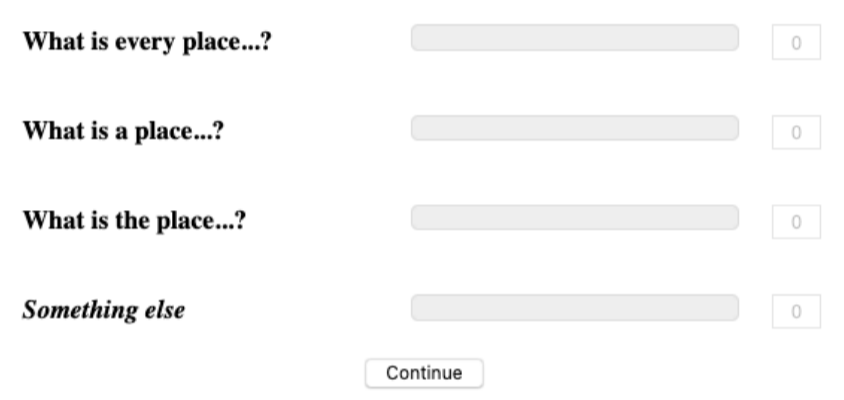
\includegraphics[scale=.52]{figures/sliders_rq.png}
\end{tcolorbox}
% \end{center}
\caption{Example trial for Root Questions task. Slider values had to sum to 100, which we rescaled to interpret ratings as a probability distribution reflecting subjective beliefs about intended meaning.}
\label{trial-ex1a}
\end{figure}


Participants were trained on four example dialogues: on two, the \emph{a}/\emph{the} paraphrases were best, and on the other two the \emph{every} paraphrase was best. We included one modal and one non-modal question for each. Further, on each training trial, participants were instructed to interpret the ellipsis in each paraphrase relative to the content in the red question (to yield, e.g., ``What is every place you have skied?" for the first paraphrase in \figref{trial-ex1a}).\footnote{Procedure, materials, analyses and exclusions were pre-registered at \url{https://bit.ly/3tp1FC1}.}

\subsubsection{Exclusions and preprocessing}
Questions that received higher ratings for \emph{something else} than any other option were removed (15\%). These tended to be rhetorical questions (e.g., \emph{Who knows?}, \emph{Who has the time?}, \emph{What are we becoming?}), whose interpretation is orthogonal to the question of whether \emph{wh}-questions are interpreted exhaustively. After exclusion, ratings were normalized such that for each participant and item, the three remaining slider values summed to 1.  

\subsubsection{Qualitative analysis}
Because this is a novel task for testing \whq interpretation, we begin by qualitatively assessing whether the ratings given for particular items accord with intuitions about the best paraphrase. 

Questions like \emph{Where do you live?} (mean=1,sd=0), \emph{Where do you work?} (.99,.03), \emph{What do you drive now?} (.99,.06), \emph{How do you spell that?} (.99,.04), \emph{When did you first take your first piano lesson?} (.92,.24), \emph{Why are you cutting off the phone?} (.81,.36)~all received mean ratings for \emph{the} at or near 1. For these questions, it is indeed possible but unlikely that there is more than one answer. 
%  karttunen \& peter 1976; \citeA{srivastav1991}). 

Questions that received high \emph{every} ratings included \emph{What does it have in it?} (.86, .31) and \emph{Where have you skied?} (.73, .37). The first occurred in a context about cooking a casserole; the second in a conversation about the hearer's love for skiing. The exhaustive interpretation---wanting to know all the ingredients in the casserole, wanting to know all the places the hearer has skied---is sensible in both cases.

% all: 102292:4, 61796:21, 87956:4; every: 101503:16, 116314:8, 
Questions that received high \emph{a} ratings often involved recommendations, e.g., \emph{What is a good brand, a inexpensive?} (.63, .39), which occurred in a discussion about computers where the hearer was an expert. Many questions involved discussions about books or movies, e.g., \emph{What have you seen lately?} (.66, .3). Other interesting cases included \emph{How can I tell you?} (.66, .42), where the speaker struggled to articulate (tell) why they like a certain movie, and \emph{What else can we talk about?} (.99, .21) where the speaker is struggling to find a conversation topic. In both cases, there are presumably multiple answers (ways to tell, things to talk about), but a single one is sufficient to achieve the speaker's goal.

Overall, the qualitative assessment of individual items suggests that participants understood the task and that the ratings are interpretable.

\subsubsection{Data analysis}

Analyses were conducted to assess overall question interpretation bias and the effect of modality and \whw on question interpretation. To this end, we conducted a mixed effects linear regression predicting critical ratings from fixed effects of \textsc{wh-word} (reference level: \emph{when}), dummy-coded and mean-centered measures of whether a modal auxiliary verb was present (\textsc{modalpresent}, 0 = not present, 1 = present) and \textsc{paraphrase} (0 = \emph{every}, 1 = \emph{a}), all 2-way interactions between fixed effects, and the 3-way interaction. We included the maximal random effects structure justified by the design: random by-item and by-subject intercepts, as well as by-item and by-subject slopes for \textsc{paraphrase}, and by-subject slopes for \textsc{wh} and \textsc{modalpresent}. 

We observed significant 3-way interactions. However, interpreting the interaction terms in this full model is very complex. We thus take the significant three-way interactions as evidence that effects varied by \whw and report the outcome of separate specific models on each \whw subset of the data: each model included fixed effects of \textsc{paraphrase}, \textsc{modalpresent}, and their interaction, coded as in the full model. 

% EXPERIMENT 1a COEFFICIENT TABLE
\begin{table}[p!]
\begin{center} 
\caption{Coefficient table (predicted $\beta$ coefficient, standard error $SE$, $t$ value, and $p$ value) for \whw-specific models in Experiment 1a. Both predictors are dummy-coded and centered (0 is no Modal Present and \emph{every}-paraphrase, 1 for Modal is present and \emph{a}-paraphrase.} 
\label{sub-model_res_ex1a} 
% \vskip .12in
\begin{tabular}{l|lllll} 
\toprule
Wh-Word & {} & $\beta$ & $SE$ & $t$ & $p$\\
\midrule
WHAT & Intercept & .25 & .006 & 38.74 & $<$.0001\\
{} & ModalPresent & .09 & .02 & 4.76 & $<$.0001\\
% \rowcolor{Gainsboro!100}
{} & Paraphrase & -.04 & .01 & -3.13 & $<$.002\\
% \rowcolor{Gainsboro!100}
{} & ModalPresent:Paraphrase & .09 & .03 & 2.8 & $<$.006\\
\bottomrule
\toprule
% HOW & $\beta$ & $SE$ & $t$ & $p$\\
% \midrule
HOW & Intercept & .20 & .01 & 24.63 & $<$.0001\\
{} & ModalPresent & .08 & .02 & 3.62 & $<$ .0005\\
% \rowcolor{Gainsboro!100}
{} & Paraphrase & .06 & .02 & 4.02 & $<$.0001\\
% \rowcolor{Gainsboro!100}
{} & ModalPresent:Paraphrase & .15 & .04 & 3.89 & $<$.0002\\
% \bottomrule
\toprule
% WHERE & $\beta$ & $SE$ & $t$ & $p$\\
% \midrule
WHERE & Intercept & .13 & .01 & 9.35 & $<$.0001\\
{} & ModalPresent & -.03 & .08 & -.37 & .72\\
% \rowcolor{Gainsboro!100}
{} & Paraphrase & -.01 & .02 & -.43 & .6\\
% \rowcolor{Gainsboro!100}
{} & ModalPresent:Paraphrase & .05 & .09 & .52 & .6\\
\bottomrule
\toprule
% {} & WHY & $\beta$ & $SE$ & $t$ & $p$\\
% \midrule
WHY & Intercept & .21 & .01 & 21.57 & $<$.0001\\
{} & ModalPresent & .02 & .02 & .87 & .34\\
% \rowcolor{Gainsboro!100}
{} & Paraphrase & .06 & .02 & 2.71 & $<$.009\\
% \rowcolor{Gainsboro!100}
{} & ModalPresent:Paraphrase & .09 & .05 & 1.82 & .07\\
\bottomrule
\toprule
% WHO & $\beta$ & $SE$ & $t$ & $p$\\
% \midrule
WHO & Intercept & .2 & .03 & 7.6 & $<$.0001\\
{} & ModalPresent & .1 & .06 & 1.6 & .12\\
% \rowcolor{Gainsboro!100}
{} & Paraphrase & .04 & .05 & .79 & .43\\
% \rowcolor{Gainsboro!100}
{} & ModalPresent:Paraphrase & .2 & .11 & 1.71 & .09\\
\bottomrule
\toprule
% WHEN & $\beta$ & $SE$ & $t$ & $p$\\
% \midrule
WHEN & Intercept & .12 & .02 & 6.41 & $<$.0001\\
{} & ModalPresent & .28 & .08 & 3.5 & $<$.004\\
% \rowcolor{Gainsboro!100}
{} & Paraphrase & .15 & .03 & 5.45 & $<$.0001\\
% \rowcolor{Gainsboro!100}
{} & ModalPresent:Paraphrase & .54 & .12 & 4.71 & $<$.0002\\
\bottomrule
\end{tabular} 
\end{center} 
\end{table}


\subsubsection{Results}

\begin{figure}[h!]
\centering
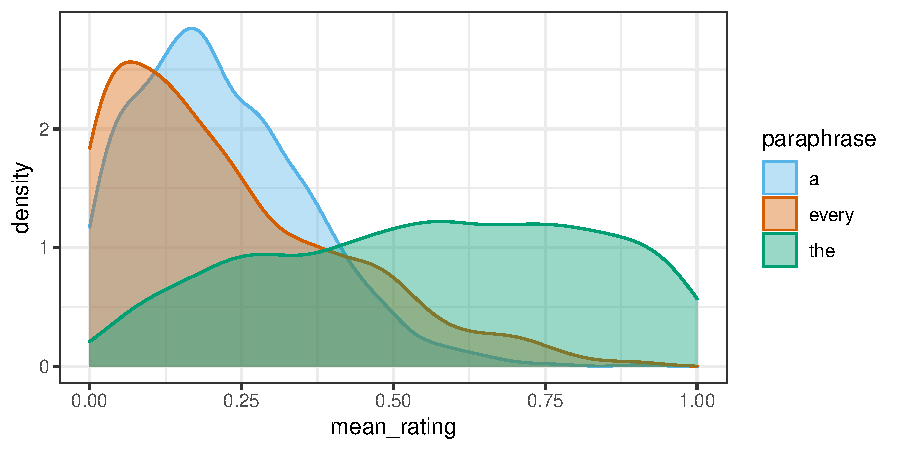
\includegraphics[scale=.8]{figures/ex1a_denisty_mean_ratings.pdf}
\caption{Mean ratings by item in Experiment 1a.}
\label{ex1a_density_mr}
\end{figure}

\begin{figure}[h!]
\centering
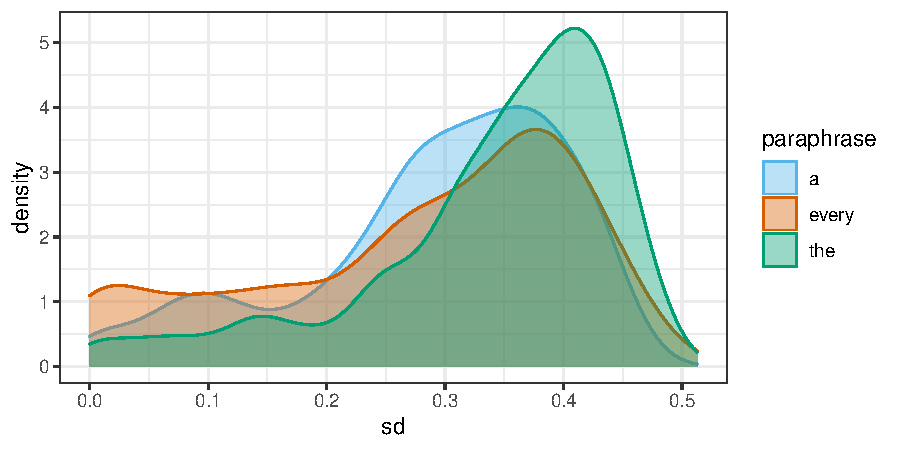
\includegraphics[scale=.8]{figures/ex1a_denisty_sd.pdf}
\caption{Standard deviations by item in Experiment 1a.}
\label{ex1a_density_sd}
\end{figure}

% \newpage
\begin{figure}[h!]
\centering
\centering
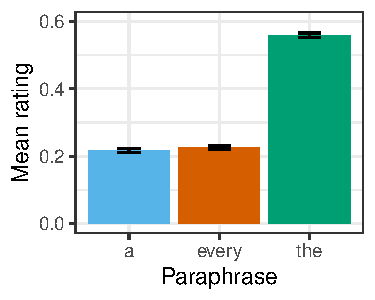
\includegraphics[scale=1]{figures/overall_rq_context.pdf}
\caption{Mean ratings by paraphrase in Experiment 1a. Here and below, error bars indicate 95\% bootstrapped confidence intervals.}
\label{ex1a_overall}
\end{figure}


\paragraph{Is there an overall MA bias?} 
\figref{ex1a_modXwh} plots mean rating as a function of Paraphrase. Rather than a preference for MA over MS readings, we observed a clear preference for the \emph{the}-paraphrase. We only observed a significant MA bias for \emph{what} questions ($\beta$=-0.04, $SE$=0.01, $t$=-3.13, $p<$0.002). In contrast, for \emph{how} ($\beta$=0.06, $SE$=0.02, $t$=4.02, $p<$0.0001), \emph{why} ($\beta$=0.06, $SE$=0.02, $t$=2.71, $p<$0.009) and \emph{when}-questions ($\beta$=0.15, $SE$=0.03, $t$=5.47, $p<$0.0001) we saw significant MS biases. Finally, for \emph{where} and \emph{who} there were no significant biases in either direction. 

\begin{figure}[h!]
\centering
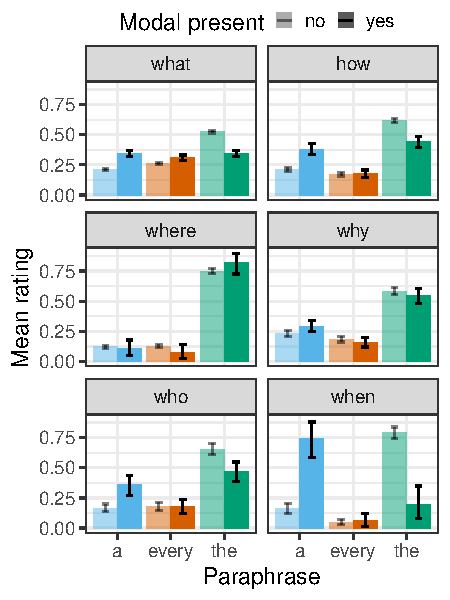
\includegraphics[scale=1]{figures/modxwh_rq_context.pdf}
\caption{Mean ratings by paraphrase, \whw and modality in Experiment 1a. Error bars indicate 95\% bootstrapped confidence intervals.} 
\label{ex1a_modXwh}
\end{figure}


\subsubsection{Q2: Do modality and \whw modulate question interpretation?}
Simply, yes. \figref{ex1a_modXwh} presents mean ratings as a function of paraphrase and the presence of a modal, separately for each \whw. We focus the following discussion on the coefficients and $p$-values in the \tableref{sub-model_res_ex1a}.

For \emph{what} questions, the overall MA bias is inverted to an MS bias when a modal is present (note the significant positive shift in coefficient values when a modal is present).

\emph{How}, \emph{why}, and \emph{when} pattern together in showing an intitial MS bias, confirming the prediction from \citeA{ginzburg1995a} and \citeA{asherlascarides1998}. \emph{Who} and \emph{where} show no initial bias, but \emph{who} shows a preference for MS while \emph{where} for MA, in contrast to those predictions. 


Thus, the prediction that \emph{who} is biased for MA is not confirmed. Only \emph{what} displayed an MA bias. Qualitative inspection of those questions which received the highest \emph{every} ratings revealed that some of these were questions with a plural-marked complex \emph{wh}-phrase (e.g., \emph{What cities are they looking at}, .92, .15) that slipped through our initial filters. These were intended to be excluded precisely because they are expected to not be ambiguous between MS and MA. However, future work should explicitly include and test complex \emph{wh}-questions. If they really are unambiguous, then plural-marked complex questions should show a clear preference for \emph{every}, and singular-marked ones for \emph{a} (or \emph{the}).

\emph{What}, \emph{how}, and \emph{when} showed a significant increase in MS ratings in the presence of a modal. \emph{Why} and \emph{who} showed marginally significant increases in MS. For \emph{where} the results were not significant but showed a shift towards MS in the presence of modals.

In general, the presence of a modal auxiliary shifts probability away from \emph{the}-paraphrases, and redistributes it to \emph{a}-paraphrases: in \figref{ex1a_modXwh} this can be seen in the higher orange than blue \emph{a} bars accompanied by the lower orange than blue \emph{the} bars, while the changes to \emph{every} are negligible. Altogether, these results confirm the observation that modal auxiliaries facilitate MS readings. 

%%%%%%%%%%%%%%%%%%%%%%%%%%%%%%%%%%%%%%%%%%%%%%%%%
\subsection{Experiment 1b: Embedded questions with context}
%%%%%%%%%%%%%%%%%%%%%%%%%%%%%%%%%%%%%%%%%%%%%%%%%

\subsubsection{Method}

\paragraph{Participants}
On Prolific, we recruited \mm{1073--is this right?} speakers who were paid about \$14/hr for their work. Eligible participants had to be born and currently reside in the US, as well as speak English as their first language. We included an addition question at the end of the study about native languages, and excluded 25 participants who reported native languages other than English. We additionally removed 37 participants for failing 2 out of 6 control trials.

\paragraph{Procedure and materials}
The procedure and materials were nearly identical to that of Experiment 1a, except in two respects. Figure \figref{trial-ex1b}.

First, the materials were embedded questions from the Switchboard corpus rather than root question. The 1075 embedded question database was divided into 35 lists of 30 questions, and 1 list of 35 questions. The distribution of \whws and modals was kept roughly proportional to the overall distribution.

Second, and in virtue of the first difference, the task itself changed in two ways. First, participants responded to the question, \emph{Based on the question in red, how likely do you think it is the that speaker means each of the following?}. Second, the paraphrases included ellipses before the \whw as well, to indicate that the paraphrase involved the lingusitic content occuring prior to the \whw.

\begin{figure}%[H]
% \begin{center}
\begin{tcolorbox}[colback=white]

\textbf{Speaker $\#$2}: \\
\textbf{Speaker $\#$1}: um.\\
\textbf{Speaker $\#$2}: so. well, uh, did you hear about that killeen massacre or whatever?\\
\textbf{Speaker $\#$1}: yeah, the, did it happen at a cafeteria or something?\\
\textbf{Speaker $\#$2}: yeah, right. that kind of i mean it just makes \color{red}you wonder \textbf{how people get guns}\color{black}\\

\noindent \emph{Based on the sentence in red, how likely do you think it is that the speaker means each of the following?}\\

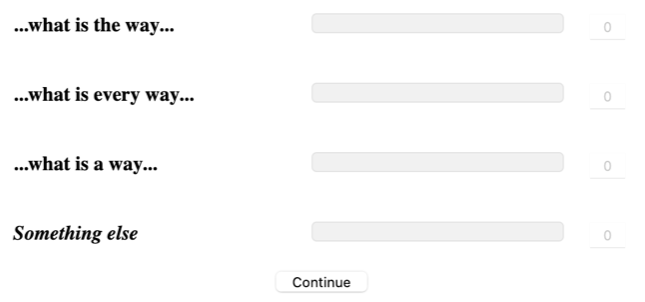
\includegraphics[scale=.5]{figures/sliders_eq.png}
\end{tcolorbox}
% \end{center}
\caption{Example trial for Embedded Questions task. Slider values had to sum to 100, which we rescaled to interpret ratings as a probability distribution reflecting subjective beliefs about intended meaning.}
\label{trial-ex1b}
\end{figure}

\subsubsection{Exclusions and preprocessing}
\mm{what is the equivalent of a rhetorical question in embedded cases?}
Questions that received higher ratings for \emph{something else} than any other option were removed (15.5\%). These are questions like \emph{but they do read. uh, where a lot of people don't have any interest in it at all}, \emph{they're real liberal now and to where probably fifty or a hundred years ago, um, the democrat party being liberal like they are?}, \emph{but i like that where they run tense} whose interpretation is orthogonal to the question of whether \emph{wh}-questions are interpreted exhaustively. After exclusion, ratings were normalized such that for each participant and item, the three remaining slider values summed to 1.  

\subsubsection{Qualitative analysis}
Because this is a novel task for testing \whq interpretation, we begin by qualitatively assessing whether the ratings given for particular items accord with intuitions about the best paraphrase.

Questions like 
\emph{I know who you’re talking about} (.94,.13), 
\emph{Do you know who the guy was that was playing the wagon driver?} (.95,.14), 
\emph{My mother taught me how to make it} (.93,.2), and
\emph{I forget how she got it} (.86,.14) 
all received high mean ratings for \emph{the}-paraphrase. For these questions, it is again possible but unlikely that there is more than one answer.

Questions that received a high rating for the \emph{every}-paraphrase included 
\emph{So He knew who worked there} (.79,.35), 
\emph{I have got to be so much more careful with what I do} (.77,.35), 
% \emph{And then we have a local rag here in town that I pick up periodically and read just to see what's going on in our little community.} (.77,.34), and
\emph{Nobody can predict what's going to happen in twenty years.} (.69,.38).
In the first case, the preceeding discourse context included an explicit domain restriction (\emph{there's only a few people that worked there}), making an MA reading possible. The second question occurs in a context about an injury, where the necessissity for caution requires MA. Finally, the third question occurs in the context of planning for possible events so an \emph{every} reading is salient.

Questions that received a high rating for the \emph{a}-paraphrase included
\emph{I’m not real sure why anybody would need a full automatic weapon} (.61,.4), 
\emph{I don’t know how to make it better for them} (.57,.4), and 
\emph{I don’t know when I’m going to get them all} (.49,.4). In all these three cases, an MS interpretation is sufficient to achieve the speaker's goal.

Overall, the qualitative assessment of individual items suggests that participants understood the task and that the ratings are interpretable.




\subsubsection{Data analysis}
Analyses were conducted to assess overall question interpretation bias and the effect of modality and \whw on question interpretation. To this end, we conducted a mixed effects linear regression predicting rating from fixed effects of \textsc{paraphrase} (reference level: \emph{every}), \textsc{wh-word} (reference level: \emph{when}), a dummy-coded and mean-centered measure of whether a modal auxiliary verb was present (\textsc{modalpresent}), all 2-way interactions between fixed effects, and the 3-way interaction. We included the maximal random effects structure justified by the design: random by-item and by-subject intercepts, as well as by-item and by-subject slopes for \textsc{paraphrase}, and by-subject slopes for \textsc{wh} and \textsc{modalpresent}. 

We observed significant 3-way interactions. %(Wh.how x ModalPresent (MP) x Paraphrase.a (Para): $\beta$=-.45, $SE$=.2, $t$=-2.2, $p<$.05; Wh.where x MP x Para.a: $\beta$=-.51, $SE$=.23, $t$=-2.2, $p<$.05; Wh.why x MP x Para.a: $\beta$=-.47, $SE$=.21, $t$=-2.2, $p<$.05). 
However, interpreting the interaction terms in this full model is very complex because two of our predictors include $>$ 3 levels. We thus take the significant three-way interactions as evidence that effects varied by \whw and  report the outcome of separate specific models on each \whw subset of the data: each model included fixed effects of \textsc{paraphrase}, \textsc{modalpresent}, and their interaction, coded as in the full model. 

An exhaustive MA bias is evidenced as a significantly negative coefficient of the `a vs.~every' \textsc{paraphrase} contrast; a non-exhaustive MS bias as a significantly positive coefficient. An introduction or strengthening of an MS bias in the presence of a modal is evidenced in a significantly positive interaction of \textsc{modalpresent} with the `a vs.~every' \textsc{paraphrase} contrast. The results of each model are shown in \tableref{sub-model_res_ex1b}, with the two relevant contrasts highlighted in gray.

% EXPERIMENT 1b COEFFICIENT TABLE
\begin{table}[p!]
\begin{center} 
\caption{Coefficient table (predicted $\beta$ coefficient, standard error $SE$, $t$ value, and $p$ value) for \whw-specific models in Experiment 1b. Both predictors are dummy-coded and centered (0 is no Modal Present and \emph{every}-paraphrase, 1 for Modal is present and \emph{a}-paraphrase.} 
\label{sub-model_res_ex1b} 
% \vskip .12in
\begin{tabular}{l|lllll} 
\toprule
Wh-Word & {} & $\beta$ & $SE$ & $t$ & $p$\\
\midrule
WHAT & Intercept & .26 & .01 & 22.85 & $<$.0001\\
{} & ModalPresent & .07 & .01 & 5.83 & $<$.0001\\
% \rowcolor{Gainsboro!100}
{} & Paraphrase & -.12 & .02 & -6.51 & $<$.0001\\
% \rowcolor{Gainsboro!100}
{} & ModalPresent:Paraphrase & .09 & .03 & 2.77 & $<$.006\\
\midrule
% HOW & $\beta$ & $SE$ & $t$ & $p$\\
% \midrule
HOW & Intercept & .22 & .01 & 19.21 & $<$.0001\\
{} & ModalPresent & .03 & .01 & 2.37 & $<$.02\\
% \rowcolor{Gainsboro!100}
{} & Paraphrase & .06 & .01 & 3.99 & $<$.0002\\
% \rowcolor{Gainsboro!100}
{} & ModalPresent:Paraphrase & 0.09 & .02 & 4.12 & $<$.0001\\
% \bottomrule
\midrule
% WHERE & $\beta$ & $SE$ & $t$ & $p$\\
% \midrule
WHERE & Intercept & .21 & .02 & 13.69 & $<$.0001\\
{} & ModalPresent & 0.03 & 0.03 & 1.09 & .28\\
% \rowcolor{Gainsboro!100}
{} & Paraphrase & .01 & .03 & .22 & .83\\
% \rowcolor{Gainsboro!100}
{} & ModalPresent:Paraphrase & .2 & .08 & 2.42 & $<$0.02\\
\midrule
% {} & WHY & $\beta$ & $SE$ & $t$ & $p$\\
% \midrule
WHY & Intercept & .19 & .01 & 27.9 & $<$.0001\\
{} & ModalPresent & 0.07 & .02 & 4.06 & $<$.0002\\
% \rowcolor{Gainsboro!100}
{} & Paraphrase & .05 & .02 & 2.42 & $<$.05\\
% \rowcolor{Gainsboro!100}
{} & ModalPresent:Paraphrase & .1 & .04 & 2.51 & $<$.02\\
\midrule
% WHO & $\beta$ & $SE$ & $t$ & $p$\\
% \midrule
WHO & Intercept & .25 & .02 & 12.08 & $<$.0001\\
{} & ModalPresent & .08 & .07 & 1.15 & .26\\
% \rowcolor{Gainsboro!100}
{} & Paraphrase & -.05 & .06 & -.82 & .42\\
% \rowcolor{Gainsboro!100}
{} & ModalPresent:Paraphrase & -.01 & .14 & -.04 & .99\\
\midrule
% WHEN & $\beta$ & $SE$ & $t$ & $p$\\
% \midrule
WHEN & Intercept & .23 & .04 & 6.37 & $<$.0001\\
{} & ModalPresent & .03 & .06 & .51 & .62\\
% \rowcolor{Gainsboro!100}
{} & Paraphrase & .12 & .06 & 2.05 & .07\\
% \rowcolor{Gainsboro!100}
{} & ModalPresent:Paraphrase & .14 & .14 & 1.05 & .31\\
\bottomrule
\end{tabular} 
\end{center} 
\end{table}

\subsubsection{Results}

\begin{figure}[h!]
\centering
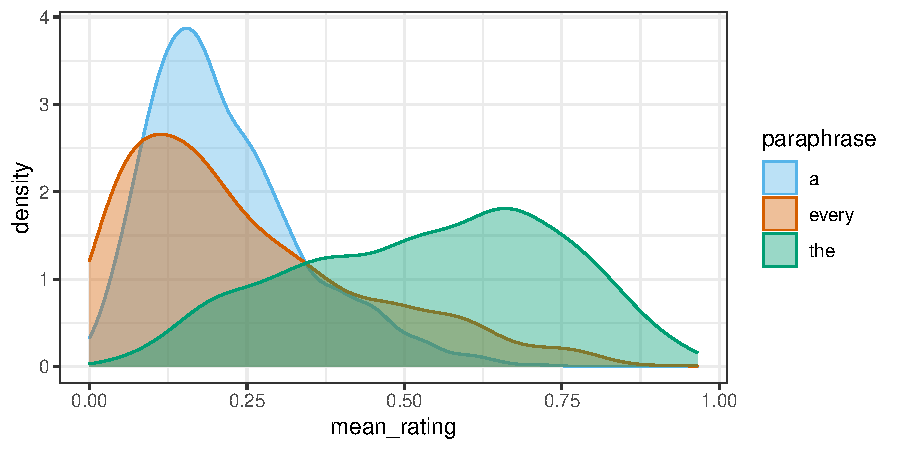
\includegraphics[scale=1]{figures/ex1b_denisty_mean_ratings.pdf}
\caption{Mean ratings by item for \emph{a}- and \emph{every}-paraphrases in Experiment 1b.}
\label{ex1b_density_mr}
\end{figure}

\begin{figure}[h!]
\centering
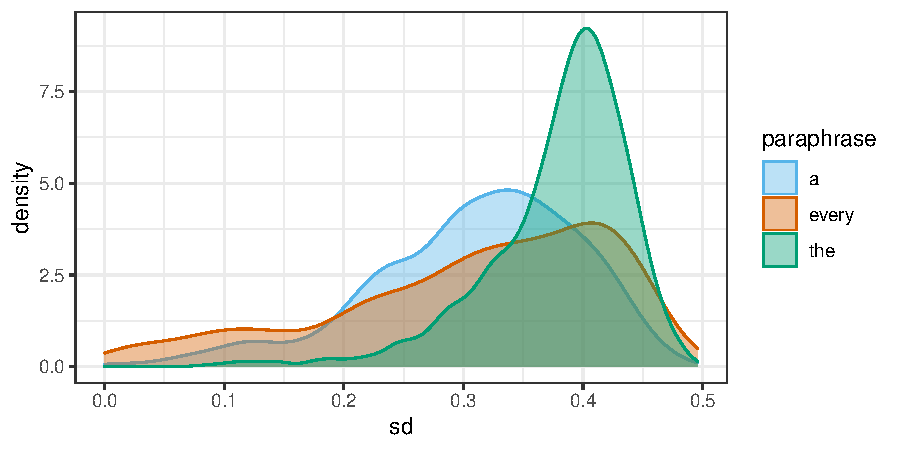
\includegraphics[scale=1]{figures/ex1b_denisty_sd.pdf}
\caption{SD by item for \emph{a}- and \emph{every}-paraphrases in Experiment 1b.}
\label{ex1b_density_sd}
\end{figure}

\begin{figure}[h!]
% \begin{subfigure}[b]{\columnwidth}
\centering
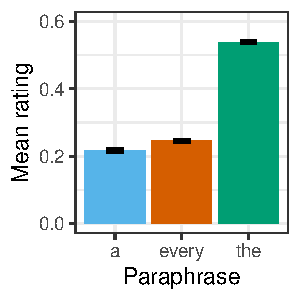
\includegraphics[scale=1]{figures/overall_eq_context.pdf}
\caption{Mean ratings by paraphrase in Experiment 1b. Here and below, error bars indicate 95\% bootstrapped confidence intervals.}
\label{ex1b_overall}
\end{figure}


\paragraph{Is there an overall MA bias?}
\figref{ex1b_overall} plots mean rating as a function of Paraphrase. We found evidence for a significant MA bias with \emph{what}-questions ($\beta$=-.12, $SE$=.02, $t$=-6.51, $p<$0.0001), and a non-significant preference for MA with \emph{who}-questions ($\beta$=-.05, $SE$=.06, $t$=-.82, $p$=.99). The remaining \whqs revealed either significant bias (\emph{how}: $\beta$=.06, $SE$=.01, $t$=3.99, $p<$0.0002; \emph{why}: $\beta$=.05, $SE$=.02, $t$=2.42, $p<$0.05) or preference (\emph{where}: $\beta$=.01, $SE$=.03, $t$=.22, $p$=.83; \emph{when}: $\beta$=.12, $SE$=.06, $t$=2.05, $p<$0.07) for MS. 

\begin{figure}[h!]
\centering
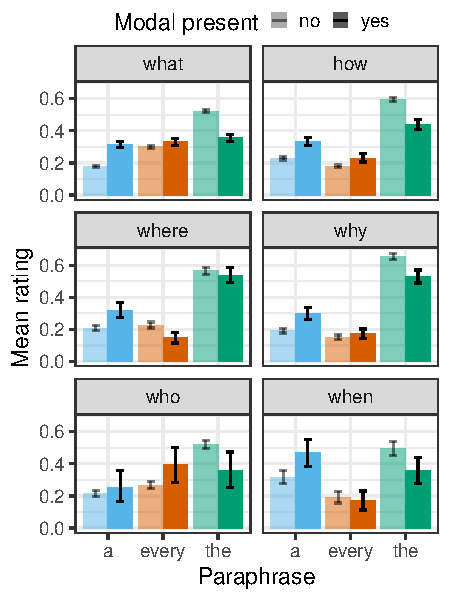
\includegraphics[scale=1]{figures/modxwh_eq_context.pdf}
\caption{Mean ratings by paraphrase, \whw and modality in Experiment 1b. Error bars indicate 95\% bootstrapped confidence intervals.} 
\label{ex1b_modXwh}
\end{figure}

\paragraph{Is MS interpretation modulated by linguistic form?}
Yes. \figref{ex1b_modXwh} plots mean rating as a function of ModalPresent, Wh-Word and Paraphrase. Interestingly, the presence of a modal significantly reversed the initial MA bias for \emph{what}- questions ($\beta$=0.09, $SE$=0.03, $t$=2.77, $p<$0.006), but only attenuated the MA preference in \emph{who}-questions. The remaining \whqs patterned together, the presence of a modal strengthened the MS bias significantly (except for \emph{when}-questions, where the effect did not reach significance).

\figref{ex1b_matrix_verbs} presents several matrix verbs that are of theoretical interest. Unfortunately, we encounter a sparse data problem for most of these verbs so we focus on \emph{know}. \figref{ex1b_modXwh_know} plots mean rating as a function of Paraphrase, Wh-Word and Modality. We found significant 2-way interactions between Wh-Word and Paraphrase in \emph{know-wh}: a significant MA bias for \emph{know-what} ($\beta$=-.09, $SE$=0.02, $t$=-4.75, $p<$0.0001) and a non-significant MA preference for \emph{know-who} ($\beta$=-.1, $SE$=0.06, $t$=-1.77, $p$=0.09), while a signfifcant MS bias for \emph{know-how} ($\beta$=.08, $SE$=.02, $t$=4.12, $p<$0.0001) and \emph{know-when} ($\beta$=0.22, $SE$=0.09, $t$=2.41, $p<$0.05), and non-significant MS preference for \emph{know-where}, \emph{know-why}.

The addition of a modal either reversed an MA bias (\emph{what}: $\beta$=0.12, $SE$=0.04, $t$=2.74, $p<$0.007) or strengthed the MS bias (\emph{know}: $\beta$=0.01, $SE$=0.03, $t$=2.93, $p<$0.005, \emph{where}: $\beta$=0.26, $SE$=0.01, $t$=2.58, $p<$0.03, \emph{why}: $\beta$=0.19, $SE$=0.07, $t$=2.49, $p<$0.02). However, there was no effect of modal for \emph{know-who}, \emph{know-when} questions.

\begin{figure}[h!]
\centering
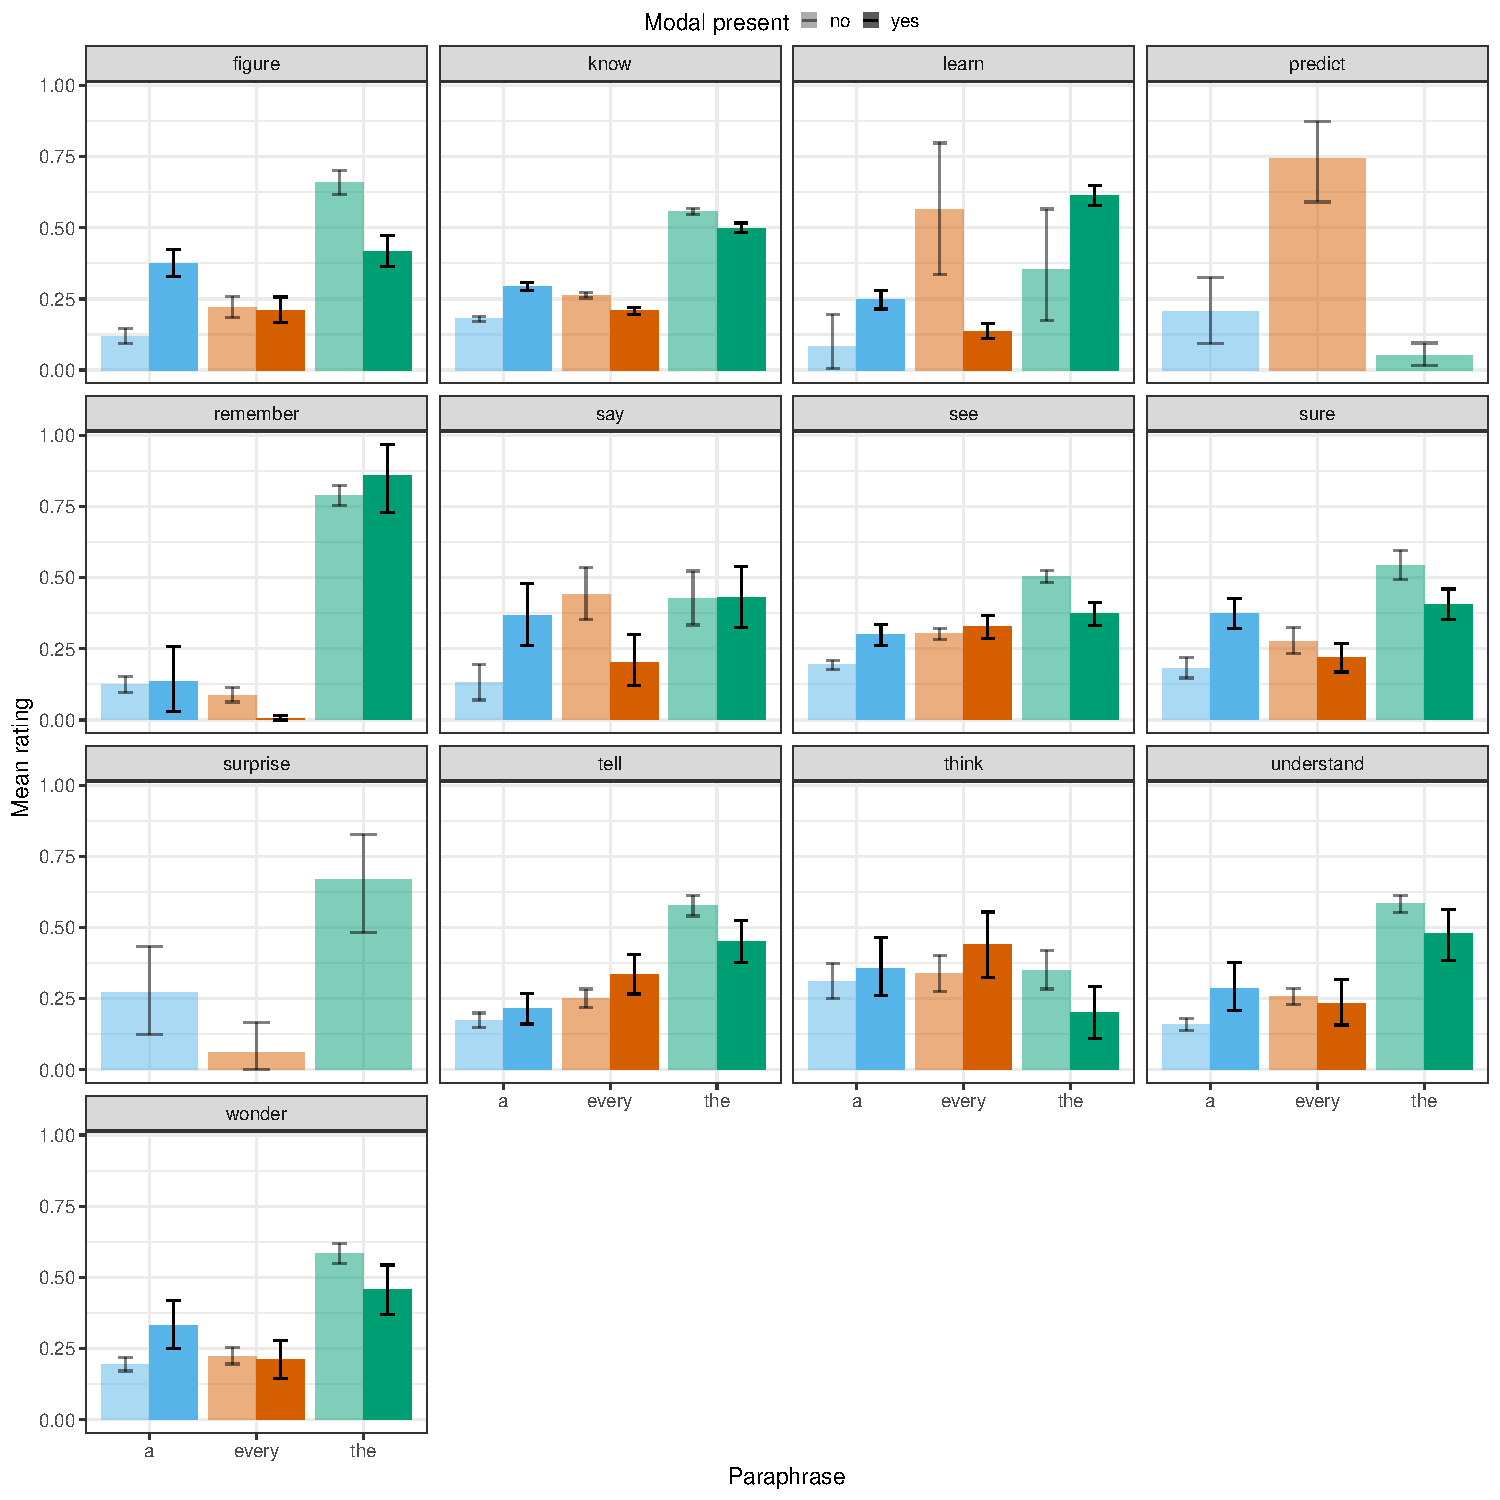
\includegraphics[scale=.6]{figures/matrixverbs_threotical_context.pdf}
\caption{Mean ratings by paraphrase for several Matrix Verbs that have been of interest in the theoretical literature, in Experiment 1b. Error bars indicate 95\% bootstrapped confidence intervals.} 
\label{ex1b_matrix_verbs}
\end{figure}


\begin{figure}[h!]
\centering
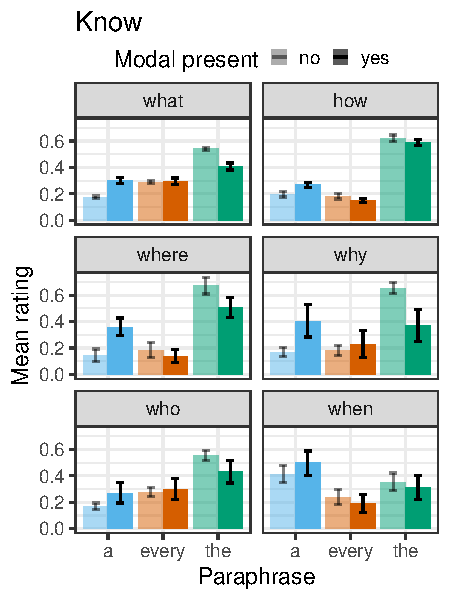
\includegraphics[scale=1]{figures/modwh_know_context.pdf}
\caption{Mean ratings by paraphrase, \whw and modality for questions embedded under \emph{know} in Experiment 1b. Error bars indicate 95\% bootstrapped confidence intervals.} 
\label{ex1b_modXwh_know}
\end{figure}

\subsection{Discussion}

Given our results, we conclude that indeed the MS reading of \emph{wh}-questions is modulated by various linguistic factors. Figure \figref{exs1_density} plots the distribution of mean ratings by item and by linguistic factors. As is clear from the plots, there is immese variation in interpretation.

\begin{figure}[h!]
\centering
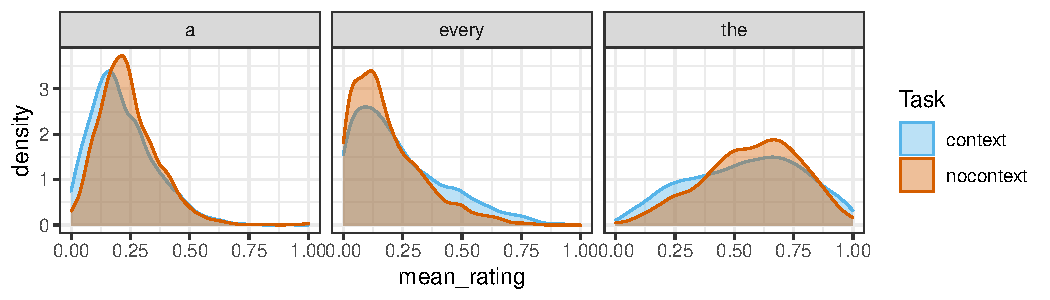
\includegraphics[scale=1]{figures/denisty_context_ratings.pdf}
\caption{Mean ratings by item for \emph{a}- and \emph{every}-paraphrases, across Experiments 1a and 1b.} 
\label{exs1_density}
\end{figure}


% \begin{figure}[h!]
% \centering
% 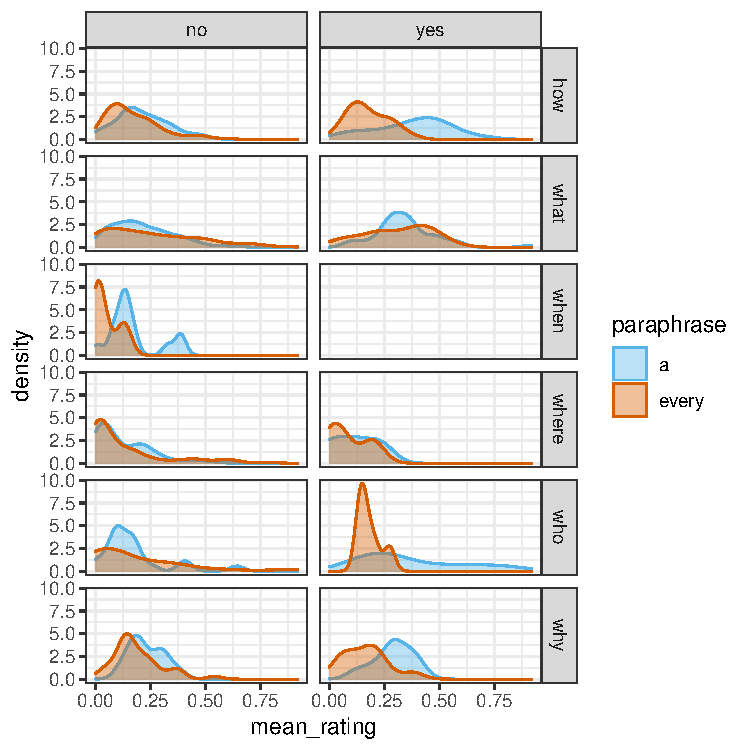
\includegraphics[scale=1]{figures/denisty_mean_ratings_factors.pdf}
% \caption{Mean ratings by item for \emph{a}- and \emph{every}-paraphrases, across Experiments 1a and 1b.} 
% \label{exs1_factors_density}
% \end{figure}

The most robust finding is that the presence of a modal significantly increases ratings for MS than the absence. This effect held even though we grouped both necessity and possibility modals together. Looking more deeply at the distribution of readings with particular modals, \mm{add some discussion about modality here, possibility versus necessisity}



There were some slight differences between the two experiments. While there was no overall MA bias for root questions, there was more of a bias in embedded questions. In both cases, however, ratings were significantly modulated by the Wh-word and the presence of modality. 


\mm{were the differences in the two experiments driven by know-wh? like, can we attribute the preference for MA in experiment 1b to know-wh? How would we test that? Can we test a model on the 1b data making a dummy coded variable for know-wh versus everything else?}


% \mm{conclusion: MS modulated by various LF factors...maybe brief discussion of sematnics theories. We also see no overall MA bias....want to show that there's lots variability in interpretation with HISTOGRAMS OF THE EVERY AND THE A REATINGS MEAN-BY-ITEM}










%%%%%%%%%%%%%%%%%%%%%%%%%%%%%%%%%%%%%%%%%%%%%%%%%
%%%%%%%%%%%%%%%%%%%%%%%%%%%%%%%%%%%%%%%%%%%%%%%%%
% EXPERIMENTS WITHOUT CONTEXT
%%%%%%%%%%%%%%%%%%%%%%%%%%%%%%%%%%%%%%%%%%%%%%%%%
%%%%%%%%%%%%%%%%%%%%%%%%%%%%%%%%%%%%%%%%%%%%%%%%%

\section{Experiments without context}
We've shown that there is no MA bias, but that linguistic factors like both the Wh-word and Modality can influence the distribution of interpretiatons. It's possible that, by removing the contexts of utterance we understand the extent to which \whq interpretation changes. In this second set of experiments, we conducted the same experiment with root and embedded questions above, however without the ten preceding lines of discourse.

\subsection{Predictions}

Based on observations from the literature, we expect (1) questions to be overall biased for MA, (2) Modal questions to be biased for MS, and possibly non-modal questions for MA, (3) \emph{who}-questions to be biased for MA, and others for MS. For experiment 1b with embedded questions, we predict that \emph{know-wh} will be biased for MA, but also that there may be some interactions with \whw.

Besides the predictions about overal and specific biases, we might expect differences between the Context and NoContext experiments if the discourse context provides crucial information relevant to determining the interpretation of root and embedded questions, which are underspecified for (non)-exhaustivity.

%%%%%%%%%%%%%%%%%%%%%%%%%%%%%%%%%%%%%%%%%%%%%%%%%
\subsection{Experiment 2a: Root questions without context}
%%%%%%%%%%%%%%%%%%%%%%%%%%%%%%%%%%%%%%%%%%%%%%%%%


\subsubsection{Method}

\paragraph{Participants}
656 participants, 25 removed for non-native. 51 additional participants were removed for failing controls.

\paragraph{Procedure and materials}
The procedure and materials were nearly identical to that of Experiment 1a as presented in \figref{trial-ex1a}, except participants were shown the root questions without the ten preceeding lines of discourse.


\subsubsection{Exclusions and preprocessing}
Questions that received higher ratings for \emph{something else} than any other option were removed (16.3\%). After exclusion, ratings were normalized such that for each participant and item, the three remaining slider values summed to 1.

\subsubsection{Data analysis}
Analyses were conducted to assess overall question interpretation bias and the effect of modality and \whw on question interpretation. To this end, we conducted a mixed effects linear regression predicting critical ratings from fixed effects of \textsc{wh-word} (reference level: \emph{when}), dummy-coded and mean-centered measures of whether a modal auxiliary verb was present (\textsc{modalpresent}, 0 = not present, 1 = present) and \textsc{paraphrase} (0 = \emph{every}, 1 = \emph{a}), all 2-way interactions between fixed effects, and the 3-way interaction. We included the maximal random effects structure justified by the design: random by-item and by-subject intercepts, as well as by-item and by-subject slopes for \textsc{paraphrase}, and by-subject slopes for \textsc{wh} and \textsc{modalpresent}. 



% EXPERIMENT 2a COEFFICIENT TABLE
\begin{table}
\begin{center} 
\caption{Coefficient table (predicted $\beta$ coefficient, standard error $SE$, $t$ value, and $p$ value) for \whw-specific models in Experiment 2a. Both predictors are dummy-coded and centered (0 is no Modal Present and \emph{every}-paraphrase, 1 for Modal is present and \emph{a}-paraphrase.} 
\label{sub-model_res_ex2a} 
% \vskip .12in
\begin{tabular}{l|lllll} 
\toprule
Wh-Word & {} & $\beta$ & $SE$ & $t$ & $p$\\
\midrule
WHAT & Intercept & .23 & .005 & 44.12 & $<$.0001\\
{} & ModalPresent & .08 & .01 & 5.43 & $<$.0001\\
% \rowcolor{Gainsboro!100}
{} & Paraphrase & .02 & .01 & 1.4 & .16\\
% \rowcolor{Gainsboro!100}
{} & ModalPresent:Paraphrase & .02 & .02 & .81 & .42\\
% \bottomrule
\midrule
% HOW & $\beta$ & $SE$ & $t$ & $p$\\
% \midrule
HOW & Intercept & .19 & .01 & 29.07 & $<$.0001\\
{} & ModalPresent & .05 & .02 & 2.79 & $<$.006\\
% \rowcolor{Gainsboro!100}
{} & Paraphrase & .09 & .01 & 6.27 & $<$.0001\\
% \rowcolor{Gainsboro!100}
{} & ModalPresent:Paraphrase & .07 & .03 & 2.64 & $<$.001\\
% \bottomrule
\midrule
% WHERE & $\beta$ & $SE$ & $t$ & $p$\\
% \midrule
WHERE & Intercept & .13 & .01 & 13.52 & $<$.0001\\
{} & ModalPresent & -.01 & .04 & -.19 & .85\\
% \rowcolor{Gainsboro!100}
{} & Paraphrase & .06 & .01 & 5.04 & $<$.0001\\
% \rowcolor{Gainsboro!100}
{} & ModalPresent:Paraphrase & -.1 & .06 & -1.64 & .1\\
% \bottomrule
\midrule
% {} & WHY & $\beta$ & $SE$ & $t$ & $p$\\
% \midrule
WHY & Intercept & .2 & .01 & 24.32 & $<$.0001\\
{} & ModalPresent & .03 & .02 & 1.8 & $<$.08\\
% \rowcolor{Gainsboro!100}
{} & Paraphrase & .08 & .02 & 4.78 & $<$.0001\\
% \rowcolor{Gainsboro!100}
{} & ModalPresent:Paraphrase & .06 & .04 & 1.77 & $<$.09\\
% \bottomrule
\midrule
% WHO & $\beta$ & $SE$ & $t$ & $p$\\
% \midrule
WHO & Intercept & .21 & .02 & 10.46 & $<$.0001\\
{} & ModalPresent & .03 & .05 & .62 & .54\\
% \rowcolor{Gainsboro!100}
{} & Paraphrase & .03 & .03 & 1.05 & .3\\
% \rowcolor{Gainsboro!100}
{} & ModalPresent:Paraphrase & .2 & .08 & 2.29 & $<$.03\\
% \bottomrule
\midrule
% WHEN & $\beta$ & $SE$ & $t$ & $p$\\
% \midrule
WHEN & Intercept & .11 & .02 & 5.99 & $<$.0001\\
{} & ModalPresent & .17 & .06 & 2.71 & $<$.02\\
% \rowcolor{Gainsboro!100}
{} & Paraphrase & .13 & .03 & 3.73 & $<$.003\\
% \rowcolor{Gainsboro!100}
{} & ModalPresent:Paraphrase & .04 & .12 & .29 & .77\\
\bottomrule
\end{tabular} 
\end{center} 
\end{table}



\subsubsection{Results}

\begin{figure}[h!]
\centering
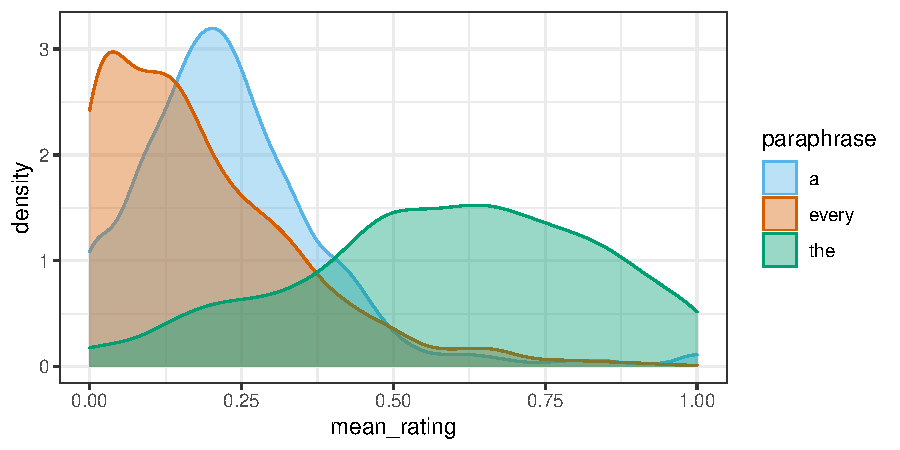
\includegraphics[scale=1]{figures/ex2a_denisty_mean_ratings.pdf}
\caption{Mean ratings by item for \emph{a}- and \emph{every}-paraphrases in Experiment 2a.}
\label{ex2a_density_mr}
\end{figure}

% \begin{figure}[h!]
% \centering
% 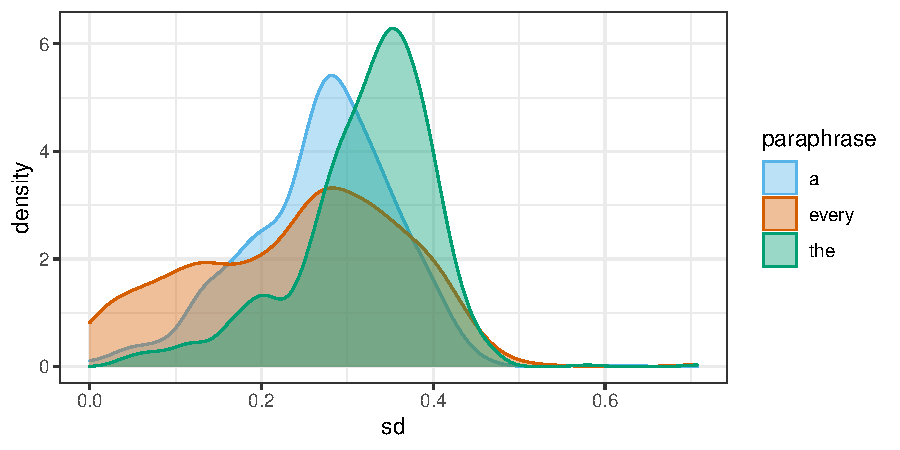
\includegraphics[scale=1]{figures/ex2a_denisty_sd.pdf}
% \caption{Mean ratings by item for \emph{a}- and \emph{every}-paraphrases in Experiment 2a.}
% \label{ex2a_density_sd}
% \end{figure}

\paragraph{Is there an overall MA bias?}

Figure \figref{ex2a_overall} plots the overal mean ratings for the three paraphrases. There were no significant biases for MA for any \whq. \emph{How}, \emph{where}, \emph{why}, \emph{when} patterned together in showing significant MS biases, while \emph{what} and \emph{who} patterned together in having positive (but not significant) coefficiants, revealing a preference towards an MS bias.
\begin{figure}[h!]
\centering
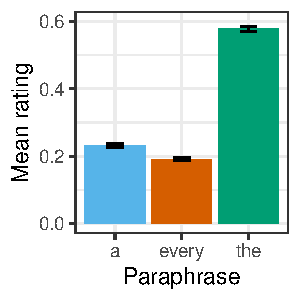
\includegraphics[scale=1]{figures/overall_nocontext_root.pdf}
\caption{Mean ratings by paraphrase in Experiment 2a. Here and below, error bars indicate 95\% bootstrapped confidence intervals.}
\label{ex2a_overall}
\end{figure}


\paragraph{Is MS modulated by linguistic form?}
\figref{ex2a_modXwh} plots mean rating as a function of ModalPresent, Wh-Word and Paraphrase. As just discussed, there were some significant differences in initial biases for MS vs. MA based on the different \whqs: \emph{how}, \emph{where}, \emph{why}, \emph{when} showed a significant MS bias, while \emph{what} and \emph{who} did not (though were positively skewed towards MS). This finding is different from the previous two studies, where at least \emph{what} and \emph{who} showed MA biases.

Given that there were no \whqs biased for MA, the presence of a modal did not significantly reverse any biases, although for \emph{when} and \emph{where} the modal appeared to neutralize the MS bias. For \emph{how}, \emph{why} and \emph{who} the interaction with modality was significant (and positively skewed towards MS), but not significant for \emph{when}.


\begin{figure}[h!]
\centering
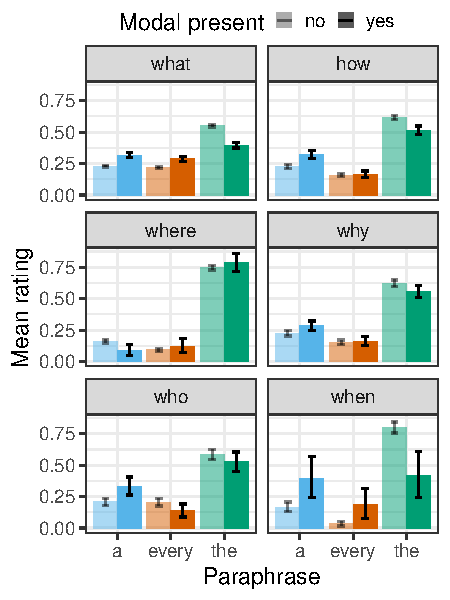
\includegraphics[scale=1]{figures/modxwh_nocontext_root.pdf}
\caption{Mean ratings by paraphrase, \whw and modality in Experiment 2a. Error bars indicate 95\% bootstrapped confidence intervals.} 
\label{ex2a_modXwh}
\end{figure}







%%%%%%%%%%%%%%%%%%%%%%%%%%%%%%%%%%%%%%%%%%%%%%%%% 
% EXPERIMENT 2b
%%%%%%%%%%%%%%%%%%%%%%%%%%%%%%%%%%%%%%%%%%%%%%%%%
\subsection{Experiment 2b: Embedded questions without context}

\subsubsection{Method}

\paragraph{Participants}
717 participants, 28 removed for non-native, 43 removed for failing controls.

\paragraph{Procedure and materials}
The procedure and materials were nearly identical to that of Experiment 2b as presented in \figref{trial-ex1b}, except--as with Experiment 2a, participants were not shown the 10 preceeding lines of discourse.


\subsubsection{Exclusions and preprocessing}
Questions that received higher ratings for \emph{something else} than any other option were removed (17.8\%). After exclusion, ratings were normalized such that for each participant and item, the three remaining slider values summed to 1.

% \subsubsection{Qualitative analysis}
% Because this is a novel task for testing \whq interpretation, we begin by qualitatively assessing whether the ratings given for particular items accord with intuitions about the best paraphrase.

\subsubsection{Data analysis}
Analyses were conducted to assess overall question interpretation bias and the effect of modality and \whw on question interpretation. To this end, we conducted a mixed effects linear regression predicting critical ratings from fixed effects of \textsc{wh-word} (reference level: \emph{when}), dummy-coded and mean-centered measures of whether a modal auxiliary verb was present (\textsc{modalpresent}, 0 = not present, 1 = present) and \textsc{paraphrase} (0 = \emph{every}, 1 = \emph{a}), all 2-way interactions between fixed effects, and the 3-way interaction. We included the maximal random effects structure justified by the design: random by-item and by-subject intercepts, as well as by-item and by-subject slopes for \textsc{paraphrase}, and by-subject slopes for \textsc{wh} and \textsc{modalpresent}. 


% EXPERIMENT 2b COEFFICIENT TABLE
\begin{table}
\begin{center} 
\caption{Coefficient table (predicted $\beta$ coefficient, standard error $SE$, $t$ value, and $p$ value) for \whw-specific models in Experiment 2b. Both predictors are dummy-coded and centered (0 is no Modal Present and \emph{every}-paraphrase, 1 for Modal is present and \emph{a}-paraphrase.} 
\label{sub-model_res_ex2b} 
% \vskip .12in
\begin{tabular}{l|lllll} 
\toprule
Wh-Word & {} & $\beta$ & $SE$ & $t$ & $p$\\
\midrule
WHAT & Intercept & .24 & .01 & 21.89 & $<$.0001\\
{} & ModalPresent & .07 & .01 & 5.76 & $<$.0001\\
% \rowcolor{Gainsboro!100}
{} & Paraphrase & -.004 & .02 & -.2 & .85\\
% \rowcolor{Gainsboro!100}
{} & ModalPresent:ModalPresent & .06 & .03 & 2.5 & $<$.02\\
\midrule
% HOW & $\beta$ & $SE$ & $t$ & $p$\\
% \midrule
HOW & Intercept & .02 & .01 & 23.86 & $<$.0001\\
{} & ModalPresent & .04 & .01 & 3.31 & $<$.002\\
% \rowcolor{Gainsboro!100}
{} & Paraphrase & .13 & .01 & 11.12 & $<$.0001\\
% \rowcolor{Gainsboro!100}
{} & ModalPresent:Paraphrase & .1 & .02 & 5.49 & $<$.0001\\
% \bottomrule
\midrule
% WHERE & $\beta$ & $SE$ & $t$ & $p$\\
% \midrule
WHERE & Intercept & .2 & .02 & 13.84 & $<$.0001\\
{} & ModalPresent & .04 & .03 & 1.36 & .18\\
% \rowcolor{Gainsboro!100}
{} & Paraphrase & .08 & .02 & 3.18 & $<$.003\\
% \rowcolor{Gainsboro!100}
{} & ModalPresent:Paraphrase & .19 & .06 & 3.23 & $<$.002\\
\midrule
% {} & WHY & $\beta$ & $SE$ & $t$ & $p$\\
% \midrule
WHY & Intercept & .18 & .01 & 22.09 & $<$.0001\\
{} & ModalPresent & .04 & .02 & 2.36 & $<$.03\\
% \rowcolor{Gainsboro!100}
{} & Paraphrase & .1 & .01 & 7.3 & $<$.0001\\
% \rowcolor{Gainsboro!100}
{} & ModalPresent:Paraphrase & .12 & .03 & 4.4 & $<$.0001\\
\midrule
% WHO & $\beta$ & $SE$ & $t$ & $p$\\
% \midrule
WHO & Intercept & .21 & .02 & 14.13 & $<$.0001\\
{} & ModalPresent & .05 & .06 & .97 & .34\\
% \rowcolor{Gainsboro!100}
{} & Paraphrase & .11 & .05 & 2.18 & $<$.05\\
% \rowcolor{Gainsboro!100}
{} & ModalPresent:Paraphrase & .05 & .1 & .51 & .61\\
\midrule
% WHEN & $\beta$ & $SE$ & $t$ & $p$\\
% \midrule
WHEN & Intercept & .25 & .02 & 10.11 & $<$.0001\\
{} & ModalPresent & .1 & .06 & 1.73 & .1\\
% \rowcolor{Gainsboro!100}
{} & Paraphrase & .18 & .05 & 3.39 & $<$.004\\
% \rowcolor{Gainsboro!100}
{} & ModalPresent:Paraphrase & .17 & .12 & 1.44 & .17\\
\bottomrule
\end{tabular} 
\end{center} 
\end{table}



\subsubsection{Results}


\begin{figure}[h!]
\centering
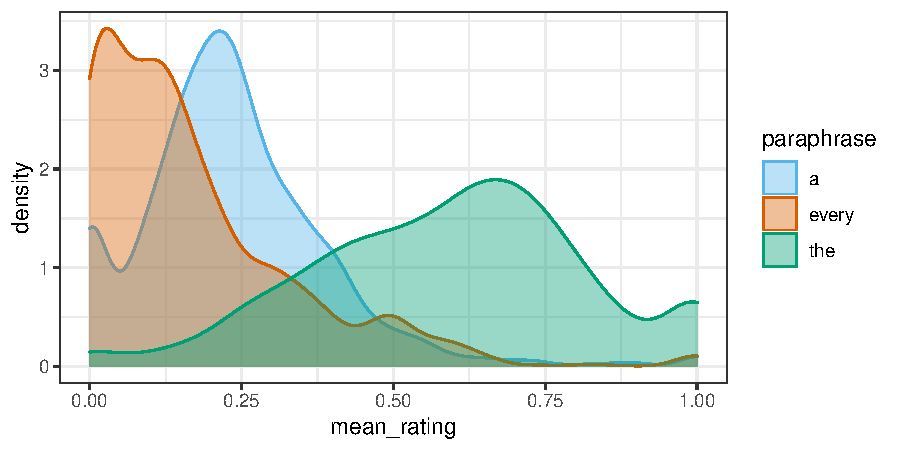
\includegraphics[scale=1]{figures/ex2b_denisty_mean_ratings.pdf}
\caption{Mean ratings by item for \emph{a}- and \emph{every}-paraphrases in Experiment 2b.}
\label{ex2b_density_mr}
\end{figure}

% \begin{figure}[h!]
% \centering
% 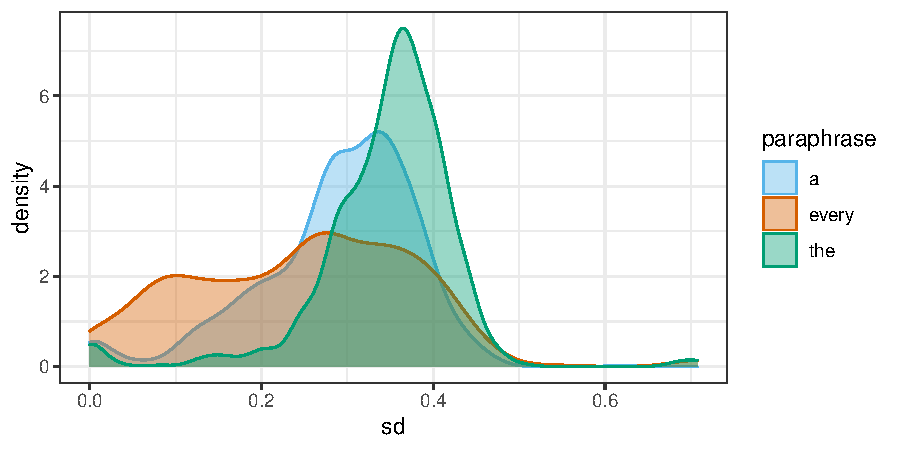
\includegraphics[scale=1]{figures/ex2b_denisty_sd.pdf}
% \caption{Standard deviations by item for \emph{a}- and \emph{every}-paraphrase in Experiment 2b.}
% \label{ex2b_density_sd}
% \end{figure}


\paragraph{Is there an overall MA bias?}
\figref{ex2b_overall} plots mean rating as a function of paraphrase. No \whq revealed a significant initial bias for MA. In contrast, all \whqs except \emph{what}-questions revealed significant initial biases for MS paraphrases. 

\begin{figure}[h!]
\centering
\centering
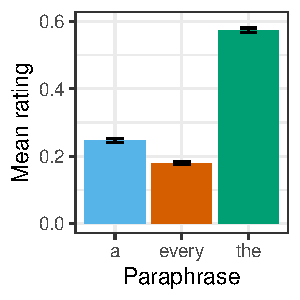
\includegraphics[scale=1]{figures/overall_nocontext_embedded.pdf}
\caption{Mean ratings by paraphrase in Experiment 2b. Here and below, error bars indicate 95\% bootstrapped confidence intervals.}
\label{ex2b_overall}
\end{figure}


\paragraph{Is MS modulated by linguistic form?}
\figref{ex2b_modXwh} plots mean rating as a function of ModalPresent, Wh-Word and Paraphrase. Unlike the previous three experiments, most questions patterned together in showing an MS bias, except \emph{what}-questions which were consistently MA skewed (although not to the point of significance). For all \whqs except \emph{when} and \emph{who}, the presence of a modal gave rise to a significant MS bias. 

\begin{figure}[h!]
\centering
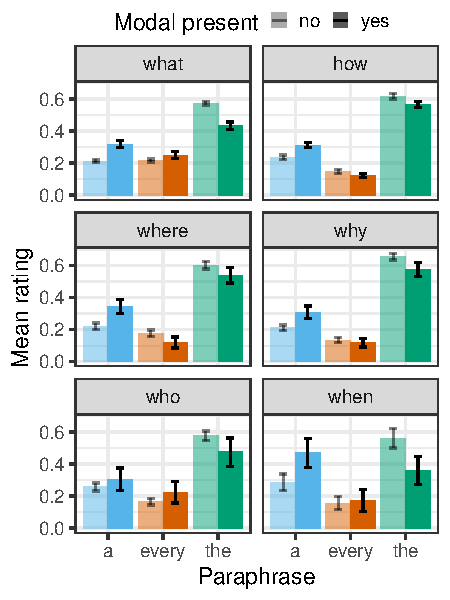
\includegraphics[scale=1]{figures/modxwh_nocontext_embedded.pdf}
\caption{Mean ratings by paraphrase, \whw and modality in Experiment 2b. Error bars indicate 95\% bootstrapped confidence intervals.} 
\label{ex2b_modXwh}
\end{figure}


\figref{ex2b_matrix_verbs} presents several matrix verbs that are of theoretical interest. As in Experiment 1b, we encounter sparse data problems and so focus on \emph{know-wh}. Before turning to those, we observe that with \emph{remember-wh}, 

\figref{ex2b_know_modXwh} presents meaning ratings for \emph{know-wh} questions as a function of paraphrase, Wh-Word and Modality. No \whq showed a bias for MA. Rather we found significant MS bias for \emph{know-how}: $\beta$=.16, $SE$=.02, $t$=8.97, $p<$0.0001 and \emph{know-where}: $\beta$=.12, $SE$=.03, $t$=3.65, $p<$0.0005; and an MS preference for \emph{know-what}, \emph{know-why}, \emph{know-who}, \emph{know-when}. The MS bias significantly increase with modality for \emph{know-what}: $\beta$=.01, $SE$=.04, $t$=3.19, $p<$0.002; \emph{know-how} $\beta$=.1, $SE$=.03, $t$=3.07, $p<$0.003, and \emph{know-where} $\beta$=.14, $SE$=.06, $t$=2.18, $p<$0.04, but not \emph{know-why}, \emph{know-who}, \emph{know-when}.

\begin{figure}[h!]
\centering
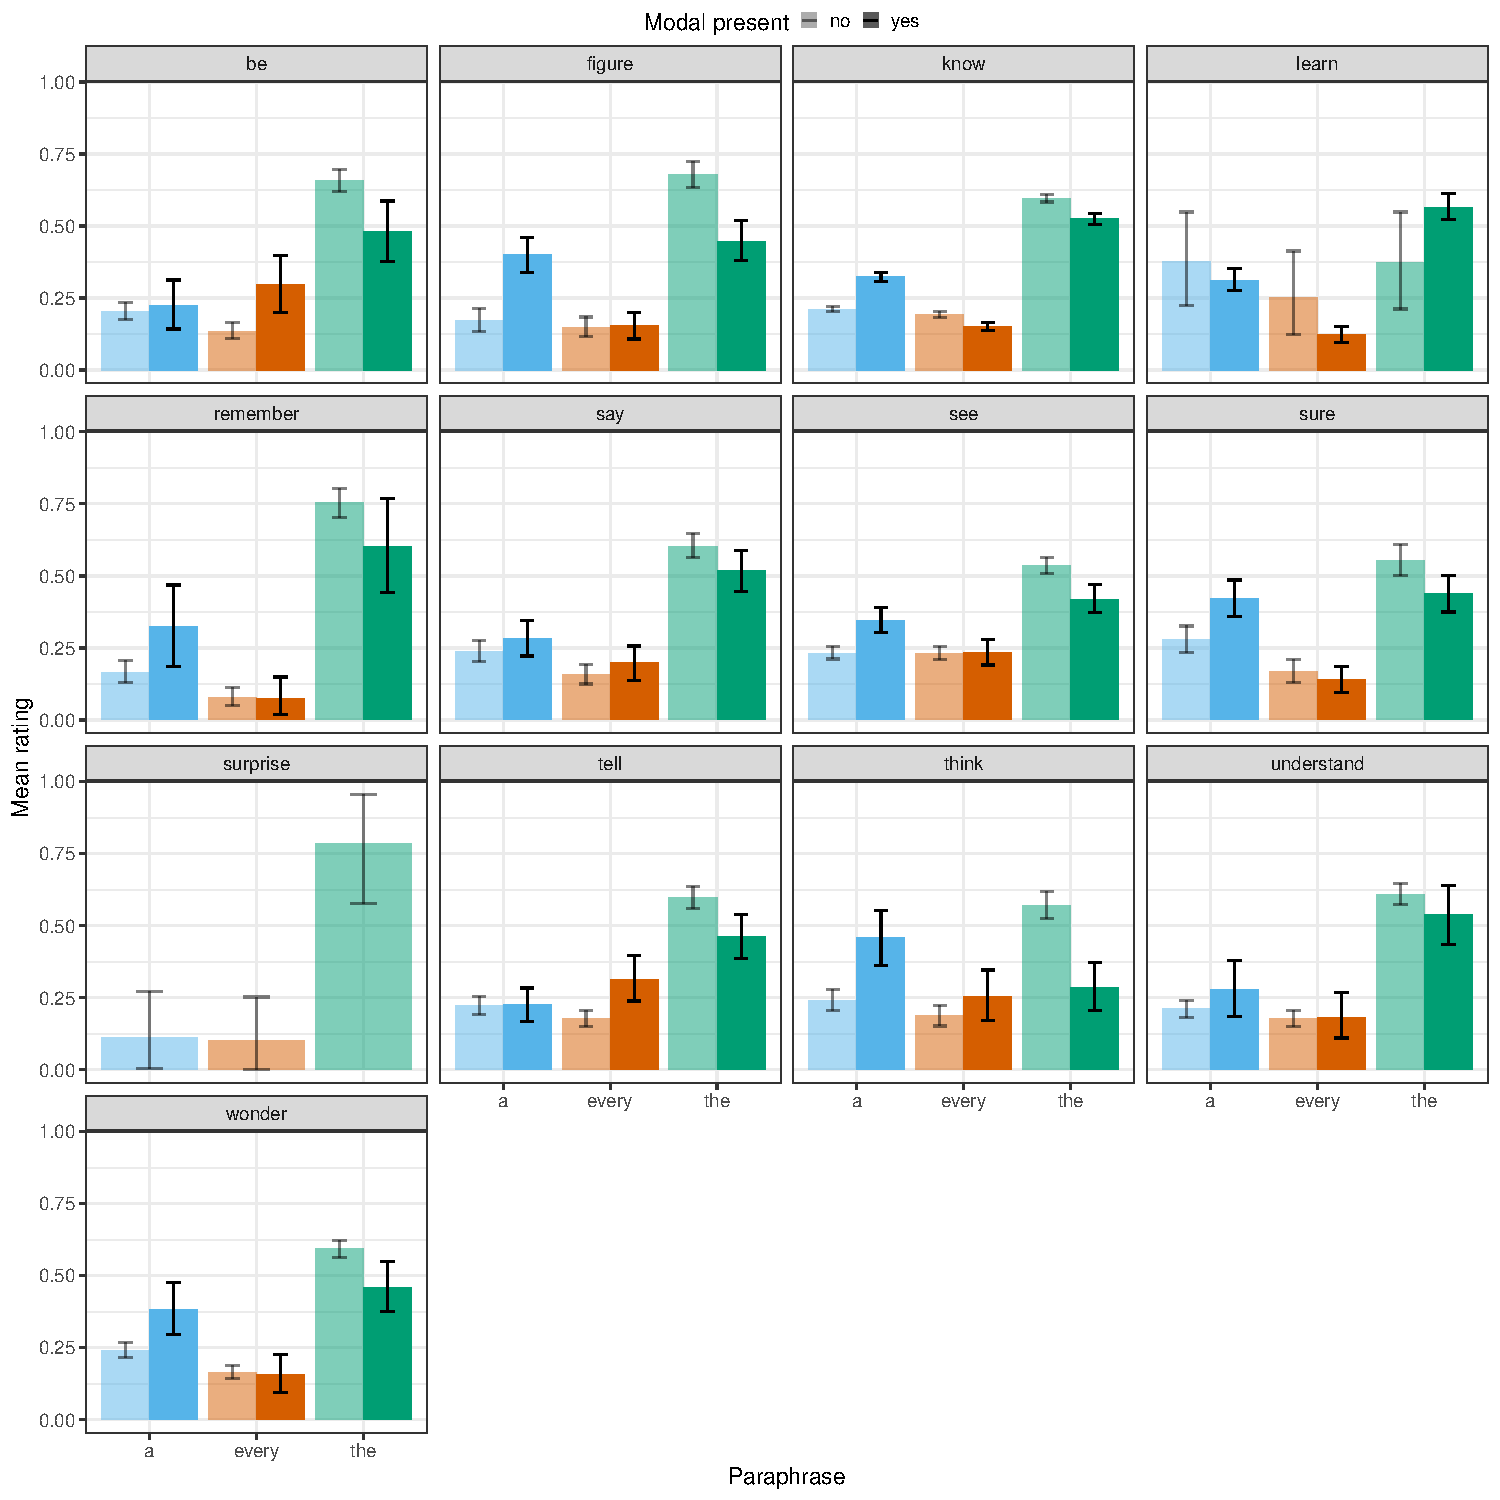
\includegraphics[scale=.6]{figures/matrixverbs_threotical_nocontext.pdf}
\caption{Mean ratings by paraphrase, \whw and modality in Experiment 2b. Error bars indicate 95\% bootstrapped confidence intervals.} 
\label{ex2b_matrix_verbs}
\end{figure}


\begin{figure}[h!]
\centering
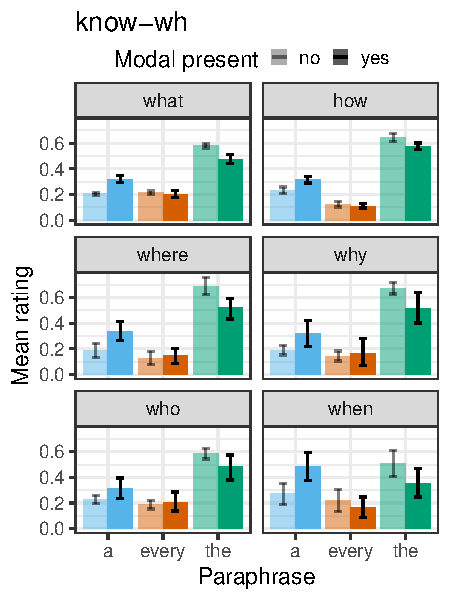
\includegraphics[scale=1]{figures/modwh_know_nocontext.pdf}
\caption{Mean ratings of questions embedded under \emph{know} as a function of paraphrase, \whw and modality in Experiment 2b. Error bars indicate 95\% bootstrapped confidence intervals.} 
\label{ex2b_know_modXwh}
\end{figure}


\subsection{Discussion}
We found that with the preceeding context removed, both root and embedded \whqs actually showed more bias for MS paraphrases than we expected. Theories which argue that only MS is context dependent would predict that MS readings should decrease without the proper contextual support. 

We still found interactions due to the lingusitic form of the question, although there were less robust effects of Modal present, as well as differences due to whether it was the root or the embedded task. For embedded \emph{what}-questions alone the presence of a modal reversed a non-significant MA bias, but there were no higher effects with root questions. For \emph{how}-questions, both root and embedded questions pattern together by exhibiting an MS bias that is strengthened by a modal. \emph{Where} and \emph{why}-questions patterned together: for root questions, there was significant MS bias but no influence of modality; for embedded questions the modal did signfifcantly increase the already significant MS bias. For root \emph{who}-questions there was only a significant interaction which raised MS ratings in the presence of modality; for embedded questions, there was significant bias for MS ratings but no effect of or interaction with modality. Finally, \emph{when}-questions showed no interactions between Paraphrase and ModalPresent, but significant positive biases for \emph{a}-paraphrases. Only with Root questions did modality boost MS.



\section{Exploratory meta analysis: Assessing the effect of context}
How crucial is the role of context? In what ways does the presence/absence of explicit linguistic context change the distribution of paraphrases? 

If the discourse context provides information about the contextual speaker goals which are crucial to resolving question interpretation, then we should find that interpretation will be harder to resolve in the NoContext condition, where that crucial information is missing. This could manifest in different ways. In the face of this uncertainty about interpretation, participants might rely more on the linguistic form of the question which provides a cue to the speaker's goal. Thus we might expect to see stronger effects of linguistic factors in the NoContext task than in the Context task. To test this, we introduce Task as a predictor in a regression model over the entire data set, allowing us to quantify the effect of Task and interaction with Wh and ModalPresent. We specifically predict that the effects of Wh and Modality should be stronger in the NoContext Task than the Context Task.

It is also possible participants will be overall more uncertaint about the intended meaning exactly because information about the speaker goal is lacking. This would be reflected in the distributions of paraphrase ratings, where in the NoContext Task the  by-item distributions would be more uniform (reflecting that uncertainty) than in Context Task. To test this hypothesis, we compared the by-item distributions for each task to the uniform distribution using the Kullback-Leibler Divergence.


% On the one hand, we might expect that without contextual information, hearers would default to the minimal model of meaning that is provided by the semantics. On the other hand, we might expect that hearers would default to their expectation about what the likely goal that the speaker who utters the sentence would have had. 

\subsection{Qualitative discussion of examples}

We subtracted, for each item and paraphrase, the rating in the Context Task from the rating in the NoContext Task. In this section, we discuss some specific examples to help us understand what the effect of context is. 


\subsubsection{Cases with a big difference from the two studies}


\paragraph{For A-paraphrases} Examples where mean rating for \emph{a}-paraphrase was higher with Context than without.

In some cases, ratings shifted clearly from \emph{a} in the context experiment to \emph{the} in the NoContext experiment.
\begin{exe}
\ex {}
Speaker A: That's awful.\\
Speaker B: And he goes out and commits it again. Fact, he's back in jail now. So, what, what, uh,\\
Speaker A: Gives you sympathy for the vigilantes.\\
Speaker B: \emph{What deterrent does he really have?} \\
\end{exe}
Rating Context [a: .626, every: .161, the: .213]
Rating Nocontext [a: .183, every: .173, the: .644]
What about the context makes a MS paraphrase better here? The context provides crucial information about what needs to be deterred. 


Some clearly went to either 'a' or 'the'/'every':
\begin{exe}
    \ex {}
    Speaker A: I mean, I'm just thinking of my circle of people that I know, I know quite a few people who have decided to not have both, both, both, uh, couples, you know, both, uh, of the parents work.\\
    Speaker B: yeah.\\
    Speaker A: and yet, uh, I, I we-, I hope to see employer based, you know, helping out. you know, child, uh, care centers at the place of employment and, and things like that, that will help out.\\
    Spealer B: uh-huh.\\
    Speaker A: \textbf{What do you think?}
\end{exe}

Rating Context [a: ..43, every: .29, the: .27]
Rating Nocontext [a: .09, every: .4, the: .5]





In other cases, there was a more even spread over the three paraphrases without context. Note that we predicted that removing context would introduce more uncertainty about the intended meanings, refelected in a flatter probability distribution in the NoContext Study. 
\begin{exe}
    \ex {}
    Speaker A: Yeah what did you think about dances with wolves when you saw it?\\
    Speaker B: Well, okay, see, we're getting back to last year. that's probably the last movie I saw. um, dances with wolves, I just adored it.\\
    Speaker A: Really?\\
    Speaker B: \textbf{How can I tell you?}
\end{exe}
Rating Context [a: ..68, every: .03, the: .29]
Rating Nocontext [a: .33, every: .23, the: .45]




\paragraph{Examples where mean rating for \emph{a}-paraphrase was higher without Context}

\begin{exe}
    \ex {}
    Speaker A: we didn't, we didn't even think about it, you know.\\
    Speaker B: No. and now, you know, what do we have now. You know, got kids that, mumblex either got a, you know, a magnum gun school, like good grief.\\
    Speaker A: r-, right.\\
    Speaker B: I mean, I'd, I'd be afraid to be in school, I mean b-, teaching, or even being a student. \textbf{and think what, what's it going to be like for my, my youngest, an my oldest son, when he goes to school?}
\end{exe}
Rating Context [a: .14, every: .59, the: .27]
Rating Nocontext [a: .77, every: .23, the: 0]


\begin{exe}
    \ex {}
\end{exe}
Rating Context [a: ., every: ., the: .]
Rating Nocontext [a: ., every: ., the: .]


\paragraph{For Every-paraphrases}

In some cases the probability mass shifted between \emph{every} and \emph{the}, and it was the Context task where \emph{every} was rated higher.
\begin{exe}
    \ex {}
    Speaker A: huh?\\
    Speaker B: \\
    Speaker A: uh-huh.\\
    Speaker B: \\
    Speaker A: I'm sure.\\
    Speaker B: Um, you look at your paycheck \textbf{and you go, oh, my gosh where did it all go?}
\end{exe}
Rating Context [a: .07, every: .75, the: .19]
Rating Nocontext [a: .21, every: .21, the: .59]
In this example, the context introduces \emph{paycheck} as the reference for \emph{it}. It is plausible that world knowledge about paychecks is to blame for the raise in the \emph{every} rating here. One doesn't spend one's paycheck (typically) at one single place, i.e., it typicallly is distributed over several places. In this sense, \emph{paycheck} isn't referring to a physical thing, but a collection of money. Note that, without the context, it makes sense that \emph{where did it all go?} would have a high \emph{the} rating, because the speaker appears to be referring to one thing going to one place. \mm{perphase, in part due to definiteness on the pronoun? find some citations like B\'uring?} The context introduces a more complex antecedent for the pronoun. \mm{It's also interesting to think about the function of \emph{all} in this example.}


\begin{exe}
    \ex {}
    Speaker A: Well, I, I, I think we did, I think we did learn some lessons that we weren't, uh, we weren't prepared for. I guess the best word would be the atrocities of war.\\
    Speaker B: Yeah.\\
    Speaker A: Uh, I mean the other wars seemed like a valiant war. I mean they seemed like a valiant thing.\\
    Speaker B: Yeah.\\
    Speaker A: \textbf{You know, you knew who was good}.
\end{exe}
Rating Context [a: .19, every: .6, the: .22]
Rating Nocontext [a: .27, every: .1, the: .63]


There actually weren't many cases where \emph{every} was higher without context. The following is an example of one, but note that the in neither task is \emph{every} rated highest. Rather, \emph{a} is rated highest in the Context Task, and \emph{the} in the No-Context task.
\begin{exe}
    \ex {}
    Speaker A: and so there's only certain times you can talk to him. and\\
    Speaker B: and you could get there and his office hours could, i mean he could have like a nine to eleven in the morning office hours and have fourty-two people waiting to talk to him, and you still didn't get to talk to him anyway.\\
    Speaker A: right, yeah.\\
    Speaker B: \textbf{well, what would be your advice to a parent of a child thinking of attening college?}
\end{exe}
Rating Context [a: .44, every: .23, the: .33]
Rating Nocontext [a: .28, every: .48, the: .24]



\paragraph{For The-paraphrases}

Cases where rating was higher in the Context task:

In most of these cases, participants were highly certain that the \emph{the} paraphrase was the one intended by the speaker in the Context experiment. In the NoContext experiment, they were less certain and we saw probability mass more evenly distributed between the three (although, often \emph{the} was still rated highest).

\begin{exe}
    \ex {}
    Speaker A: of course I would want one if somebody was given to me.\\
    Speaker B: yeah.\\
    Speaker A: but I maybe would buy a BMW. uh, or, even a Volvo.\\
    Speaker B: uh-huh.\\
    Speaker A: \\
    Speaker B: \textbf{What do you have now?}
\end{exe}
Rating Context [a: .02, every: .01, the: .96]
Rating Nocontext [a: .25, every: .26, the: .49]
In this example, Context supplies the relevant domain of cars, in which typically people only have a single one. Even though \emph{the} is still highly rated in the NoContext task, note that probability is distributed almost evenly between \emph{a} and \emph{every}. 


\begin{exe}
    \ex {}
    Speaker A: and I did not like giving it out. I mumblex gave out my work number.\\
    Speaker B: Right.\\
    Speaker A: But I think I'm not sure if it's by law just, otherwise I think the practice has basically been eliminated asking for a phone number.\\
    Speaker B: Well, that's the thing I hate too about, uh, radio shack. \\
    Speaker A: \textbf{How did radio shack work?}
\end{exe}
Rating Context [a: .03, every: .08, the: .89]
Rating Nocontext [a: .33, every: .21, the: .47]

In context, the question is clearly about policies on asking for phone numbers. Furthermore, the existential presupposition that Radio Shack has a policy on the topic is satisfied by Speaker B who explicitly has a (negatively valanced) attitude towards it. Without context, it's less clear which policy is the relevant one (i.e., \emph{work} in what respect?). It's less clear that the presuppositions of \emph{the} are satisfied, reflected in the fact that ratings for \emph{a} and \emph{every} are both higher than in the Context Task (although \emph{the} is still the highest). Participants are less confident that the \emph{the} paraphrase was the intended one. 

Cases where rating for \emph{the} was highest in the NoContext task often involved some variation on the question \emph{What do you think?}, which was often rated with an expremely high probability for \emph{the} in the NoContext task (at 1). In the Context task, probability mass was often evenly distributed between all three paraphrases.

\begin{exe}
    \ex {}
    Speaker A: yeah, that's okay.\\
    Speaker B: Well, that's what I mean like I didn't know what the diffference between Dukakis and Bush was.\\
    Speaker A: Uh-huh.\\
    Speaker B: you know, I didn't know anything about Bush or Dukakis.\\
    Speaker A: \textbf{so what do you think about, uh, what do you think about what you see on tv about them, like in the news or on the ads?}
\end{exe}
Rating Context [a: .32, every: .36, the: .32]
Rating Nocontext [a: 0, every: 0, the: 1]

\begin{exe}
    \ex {}
    Speaker A: So long.\\
    Speaker B: Thanks a lot. \\
    Speaker A: Well, uh, ho-, how do you view this whole subject?\\
    Speaker B: \\
    Speaker A: are you, uh, one who feels like you have, have benefited from the change in, in roles in women? \textbf{or, or what do you think?}
\end{exe}
Rating Context [a: .26, every: .49, the: .24]
Rating Nocontext [a: 0, every: 0, the: 1]
Here's a case where it seems the 10 preceeding lines included the end of one discussion as well as the actual discourse preceeding the target question.



\subsubsection{Cases where there was minimal change in rating between the two Tasks}

% \paragraph{For A-paraphrases}

Some cases there was no uncertainty, and no effect of context.
\begin{exe}
    \ex {}
    Speaker A: I need to make myself do that.\\
    Speaker B: Yeah. I slacked off a little because of, um, I'm about to graduate from college and so this past couple months have been really hectic so I haven't really gone and I've really been faithful these past two months of going to the health club and working out but...\\
    Speaker A: \textbf{What school you going to?}\\
\end{exe}
Rating Context [a: 0, every: 0, the: 1]
Rating Nocontext [a: 0, every: 0, the: 1]

% \paragraph{For Every-paraphrases}

\begin{exe}
    \ex {}
    Speaker A: Generally cheap things.\\
    Speaker B: uh-huh.\\
    Speaker A: \\
    Speaker B: uh-huh\\
    Speaker A: \\
    Speaker B: uh-huh. yeah \textbf{we know how that goes}.\\
\end{exe}
Rating Context [a: .18, every: .1, the: .71]
Rating Nocontext [a: .18, every: .11, the: .7]

% \paragraph{For The-paraphrases}

\begin{exe}
    \ex {}
    Speaker A: oh, yeah.\\
    Speaker B: and here's tis bum that didn't have a job.\\
    Speaker A: yeah.\\
    Speaker B: and he's got a attorney that you and i could never afford.\\
    Speaker A: that's true.\\
    Speaker B: \textbf{Who's paying for that?}\\
\end{exe}
Rating Context [a: .09, every: .07, the: .84]
Rating Nocontext [a: .09, every: .07, the: .84]





\subsection{Results}

\figref{Task_overall} presents a comparison of the overal results from the Context task compared with the NoContext task. Overall, it seems that the distribution of ratings are largely similar between the two tasks; however, means are numerically higher in the NoContext Task for both \emph{a} (NoContext: mean=0.239, sd=.309, vs. Context: 0.216, 0.331) and \emph{the}-paraphrases (NoContext: mean=0.576, sd=.387, vs. Context: 0.547, 0.432) but the opposite for \emph{every}-paraphrases (Context: 0.237, 0.366, vs. NoContext: mean=0.185, sd=.303). 



\begin{figure}[h!]
\centering
\centering
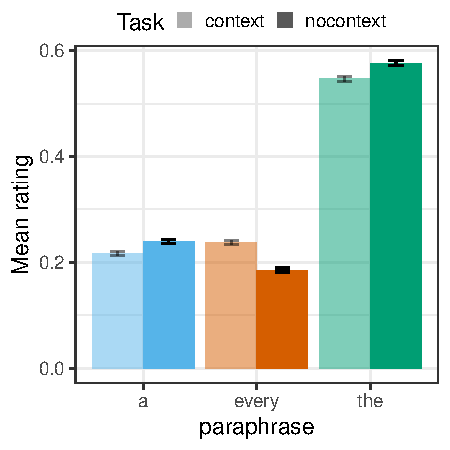
\includegraphics[scale=1]{figures/overall_Task.pdf}
\caption{Mean ratings by paraphrase comparing Context and NoContext Experiments.}
\label{Task_overall}
\end{figure}

We can see these differences from a slightly different angle in \figref{density_Task_overall}, which presents the mean by-item ratings for each paraphrase plotted as a function of Task. 
\begin{figure}[h!]
\centering
\centering
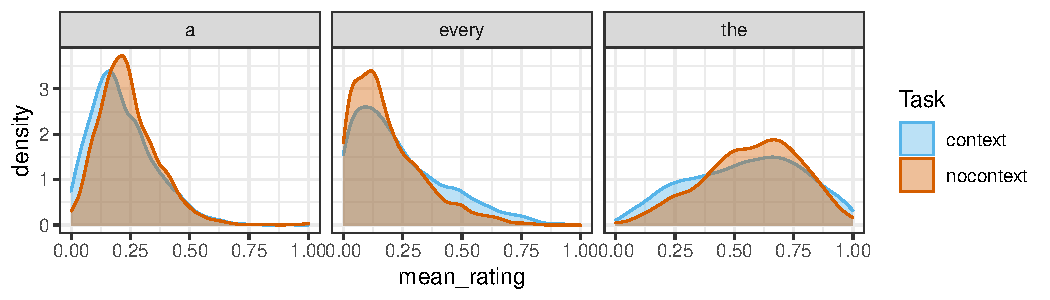
\includegraphics[scale=1]{figures/denisty_context_ratings.pdf}
\caption{Mean ratings by paraphrase comparing Context and NoContext Experiments.}
\label{density_Task_overall}
\end{figure}


\subsubsection{Regression analysis}
Some semantic theories predict that MS only requries special licensing by the context. Thus, if information that plays a licensing role is removed, it is plausible that those theories would predict that MS readings would decrease in the second set of experiments. We already saw that this prediction was not borne out. 

Analysis were conducted to assess the effect of Task (Context, NoContext) in addition to modality and \whw on question interpretation. Given the potential 4-way interaction by including Task as a predictor, we broke the data set up by Paraphrase and conducted three sub-model analysis.

% \mm{add in the model results from breaking it up by paraphrase}

\subsubsection{Quantifying information loss with KL divergence}
In addition to comparing 
We calculated the Kullback-Leibler Divergence from each Task and the uniform distribution over paraphrases to determine whether information about interpretation was lost in the NoContext Task, and conducted a regression analysis to determine whether Task predicted the KL divergence score.

We found that removing the context significantly decreased the KL-divergence score, meaning that ratings in the NoContext Task were closer to the uniform distribution, that information was lost when the context was removed.

% \mm{graph the KL divergence}

\begin{figure}[h!]
\centering
\centering
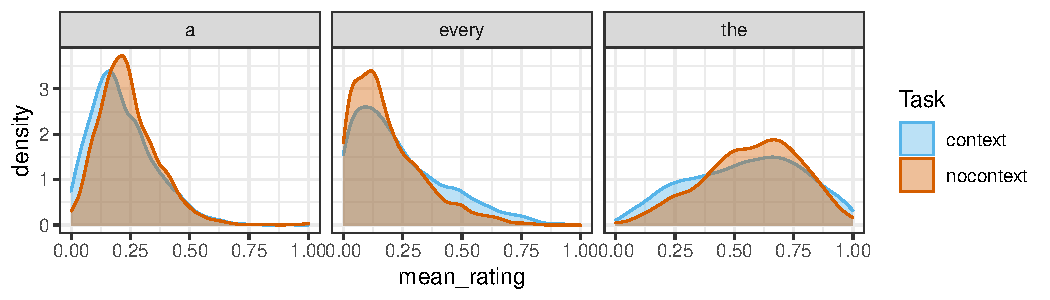
\includegraphics[scale=1]{figures/denisty_context_ratings.pdf}
\caption{Mean ratings by paraphrase comparing Context and NoContext Experiments.}
\label{density_kld_overall}
\end{figure}


\subsection{Discussion}
We found that effects of Task were significant for Wh-Word, but not for Modality, suggesting that context is informative wrt the wh-domain which importantly helps determine the meaning that the speaker intended. 


\subsection{Annotation of context for domain-relevant information}
We annotated a random sample of contexts of questions that rated high for MS for features that were relevant to determining the size and type of the \emph{wh}-domain.

\section{General Discussion}

We presented four experiments designed to test the naturalistic distribution of (non-)exhaustivity in \whqs from the Switchboard corpus of telephone conversations. Experiments 1a and 2a looked at root questions, while Experiments 1b and 2b looked at questions embedded under propositional attitude verbs. To test the effect of contextual information on interpretation, Experiments 1a/1b presented targets with the immediately preceding dialogue, while Experiments 2a/2b presented targets without.

Givn our results, we argue that the semantic representation of a question is maximally underspecified or really weak, existential in meaning. The interpretive process of resolving that underspecification is Bayesian, and involves joint reasoning about the linguistic signal and its possible alternatives, in addition to the contextual speaker's goal.



\subsection{Beyond three linguistic factors}

We highlighted three linguistic factors that have been discussed in the literature, modality, \whw, and matrix verb. However, there are other linguistic factors which we did not include in our analyses. 

\paragraph{Modality}
First, we used a coarse-grained measure of modality that included all modal auxiliaries and additionally non-finite clauses in embedded questions, ignoring variation due to modal force and flavor (\cite{kratzer1981,kratzer1991,portner2009}). The semantics literature on the effect of modality on MS typically has focused on the existential priority modal \emph{can} as it has occured in the classic example, \emph{Where can I find an Italian newspaper?} On the one hand, we might predict that any modal with existential force would allow for MS because it's the existential bit that drives the MS meaning. This would put the modal observation squarely in line with the observation about 

\paragraph{In/definiteness}
Second, definite and indefinite noun phrases may reveal interesting differences with respect to MS and MA. On the one hand, 

\paragraph{Other \emph{Wh}-phrases}
Third, we chose to include only monomorphemic \emph{wh}-phrases, and not include questions with singular or plural marked \emph{wh}-phrases. 

Similarly, we did not include clefts or relative clauses. There is a question in the literature on clefts about the extent to which they allow for non-exhaustive readings \mm{more citations?..check diss, devaug-geiss, zimmermann, destruel}.


Better that pragmatics is not sufficient: 
(discussion from George 205-206)
questions with ostensibly the same semantic representation 
\begin{exe}
\ex {}
    \begin{xlist}
        \ex Who has leprosy?
        \ex Who are some people with leprosy?
    \end{xlist}
\end{exe}
But we can question indeed whether these two questions would be asked by a speaker iwth the same goals in mind?


\paragraph{Question Type}
Fourth, we did find some differences between root and embedded questions. Embedded questions appeared to slightly prefer MA paraphrases over MS paraphrases, while root questions showed the opposite. This effect could be due to the additional effect of Matrix verb which was not present for Root Questions. Indeed, the majority of embedded questions occured with the verb \emph{know}, which is classically MA. Additionally, there were some cases of embedded questions in which the question contained subject-auxiliary inversion, a connonical root question syntax. Some have argued that MS, being pragmatic, should not be possible in embedded questions (\cite{karttunen1977}\mm{footnote 4}, \cite{groenstok1984}\mm{footnote 14}, \mm{xiang?})

Of course, this kind of ``pragmatics does not interfere in semantics'' view is less in vogue than it used to be, in part because of the growing understanding of pragmatic processing (\mm{reference list from kreiss \& degen cog sci paper}). We did an exploratory analysis on the effect of Question Type (true embedded, embedded with subject-aux inversion, true root) and the effects were not overwhelmingly different. \mm{Show graphs? do regression?} 


\paragraph{Corpus Genre}
The Switchboard corpus is comprised of conversational dyads between randomly assigned employees of Texas Instrunmnets. The conversants were strangers so they did't share a lot of common ground. This effected the corpus 

Already, the fact that \whq interpretation could be sensitive to all these further factors suggests that 


\section{Conclusion}

Human communication proceeds remarkably fast and effortlessly despite the rampant underspecification of speakers' utterances with respect to the meaning they intend to convey. Resolving that underspecification requires that hearers integrate a wide range of possibly uncertain linguistic and extra-linguistic cues. 

This view of pragmatics, informed by psycholinguistic research on language processing that espouses a dynamic, nonmodular view of comprehension, has provided a useful novel perspective on many phenomena at the semantics/pragmatics interface. For instance, one of the most-studied cases of underspecification in experimental pragmatics is the scalar inference from \emph{some} to \emph{not all} (e.g., \emph{Scully ate some of the cookies} typically licenses the inference that she did not eat all of them). Recent research using a large dataset of naturally-occurring utterances has revealed a large amount of variability in whether hearers derive scalar inferences \cite{degen2015}. Rather than being random, the observed variability was dependent on multiple features of the linguistic and discourse context. Data from controlled experimental tasks with artificially generated stimuli confirm these results: scalar inferences are systematically dependent on (the hearer's estimate of) the speaker's discourse goal \cite{zondervan2010}\mm{kursatdegen2020}, the speaker's epistemic state \mm{goodmanstuhlmueller2013}\cite{brehenyetal2013}, and which alternatives are contextually available \cite{huangsnedeker2011,degentanenhaus2016}, among other cues. These results were unexpected in light of the theoretical literature, which had predicted a higher prevalence of the inference and no systematic context-dependence \cite{levinson2000}.

A good deal of experimental attention has been paid to pragmatic inferences, like scalar inferences, that are the result of reasoning about declarative utterances. In contrast, there is much less discussion about the cues guiding hearers' interpretation of non-declarative utterances like questions. Consider polar (\emph{yes}-\emph{no}) questions: these can be answered literally with a \emph{yes} or \emph{no}, but often the literal answer is neither the most appropriate, nor what the speaker intended. In \citeA{searle1975}'s classic example, a dinner guest who asks \emph{Can you reach the salt?}~likely intends you to pass the salt, not say \emph{yes}. Whether a hearer understands the speaker to want a literal or non-literal answer depends on what they infer about the speaker's goals. \citeA{clark1979} surveyed liquor merchants to determine how they answered a polar question like \emph{Does a fifth of Jim Beam cost more than \$5?} when it was introduced by a brief sentence that made the speaker's goal explicit. If the speaker first stated \emph{I want to buy some bourbon}, merchants were more likely to answer with the exact price of the whiskey. If the speaker instead stated \emph{I've got \$5 to spend}, merchants were more likely to provide the more literal \emph{yes}/\emph{no} answer. That is, merchants responded by addressing the inferred speaker goal. Research in computational cognitive science has followed suit by modeling question asking and answering as a species of rational, goal-directed behavior \cite{hawkinsetal2015,rotheetal2018}. \mm{hawkinsgoodman2019?}\emph{Wh}-questions are even more complex than polar questions in that even their literal interpretation is underspecified. 




\bibliographystyle{apacite}

\setlength{\bibleftmargin}{.125in}
\setlength{\bibindent}{-\bibleftmargin}

\bibliography{questions}

\end{document}